%!TEX root = ../thesis.tex
%*******************************************************************************
%*********************************** Fourth Chapter ****************************
%*******************************************************************************
%*******************************************************************************
\cleardoublepage
\chapter{Kernel-based central tendency estimation}
\label{chpt:4}
%*******************************************************************************
\hfill
\localtableofcontents
\newpage

\begin{tcolorbox}[colback=gray!5!white, colframe=gray!5!white, coltitle=gray, coltext=gray, fontupper=\footnotesize, fontlower=\footnotesize, title=\textbf{Parts of this chapter are adapted from the following publication:}]
    \begin{itemize}
        \item[\ding{125}] E. Fekhari, V. Chabridon, J. Muré and B. Iooss (2024). ``Given-data probabilistic fatigue assessment for offshore wind turbines using Bayesian quadrature''. In: \textit{Data-Centric Engineering}, In press.
    \end{itemize}
\end{tcolorbox}

%============================================================%
\section{Introduction}
%============================================================%
As a sustainable and renewable energy source, offshore wind turbines (OWT) are likely to take a growing share of the global electric mix. 
However, to be more cost-effective, wind farm projects tend to move further from the coast, exploiting stronger and steadier wind resources. 
Going further offshore, wind turbines are subject to more severe and uncertain environmental conditions (i.e., wind and waves). 
In such conditions, their structural integrity should be certified. 
To do so, numerical simulation and probabilistic tools have to be used. 
In fact, according to \citet{graf_2016}, for new environmental conditions or new turbine models, international standards such as \citet{iec_2019} from the International Electrotechnical Commission and \citet{dnv_loads_2016} from Det Norske Veritas recommend performing over $2 \times 10^5$ simulations distributed over a grid. 
However, numerical simulations are computed by a costly hydro-servo-aero-elastic wind turbine model, making the design process time-consuming. 
In the following, the simulated output cyclic loads studied are aggregated over the simulation period to assess the mechanical fatigue damage at hot spots of the structure. 
To compute the risks associated with wind turbines throughout their lifespan, one can follow the steps of the universal framework for the treatment of uncertainties presented in the introduction of this manuscript \fig{fig:UQ_methodo}. 
After specifying the problem (Step A), one can quantify the uncertainties related to site-specific environmental conditions represented by the random vector $\bX \in \iD_{\bX} \subset \R^d, d\in \N^{*}$ (Step B). 
Then, one can propagate them through the OWT simulation model (Step C) denoted by $g: \iD_{\bX}\rightarrow \R, \bX \mapsto Y = g(\bX)$, and estimate a relevant quantity of interest $\psi(Y) = \psi(g(\bX))$ (e.g., a mean, a quantile, a failure probability). 
An accurate estimation of the quantity of interest $\psi(Y)$ relies on both a relevant quantification of the input uncertainty and an efficient sampling method.

Regarding Step B, when dealing with uncertain environmental conditions, a specific difficulty 
often arises from the complex dependence structure such variables may exhibit. 
Here, two cases may occur: either measured data are directly available (i.e., the ``given-data'' context) or a theoretical parametric form for the joint input probability distribution can be postulated.
Such existing parametric joint distributions often rely on prior data fitting combined with expert knowledge. 
For example, several parametric approaches have been proposed in the literature to derive such formulations, ranging from fitting conditional distributions \citealp{vanem_fekhari_2023}) to using vine copulas \citep{li_zhan_2020}. 
When a considerable amount of environmental data is available, nonparametric approaches such as the empirical Bernstein copula were studied in Chapter~\ref{chpt:3} to capture complex dependence structures. 
Alternatively, an idea is to directly use the data as an empirical representation of input uncertainties in order to avoid an additional inference error. 

Step C usually focuses on propagating the input uncertainties in order to estimate the quantity of interest. 
Depending on the nature of $\psi(Y)$, one often distinguishes between two types of uncertainty propagation: a central tendency estimation (e.g., focusing on the output mean value or the variance) and a tail estimation (e.g., focusing on a high-order quantile or a failure probability). 
When uncertainty propagation aims at central tendency estimation, the usual methods can be split into two groups. 
First, those relying on sampling, i.e., mainly Monte Carlo sampling \citep{graf_2016}, quasi-Monte Carlo sampling \citep{muller_cheng_2018}, geometrical subsampling \citep{kanner_2018_OMAE}, or deterministic quadrature rules \citep{bos_2020}. 
All these methods estimate the quantity directly on the numerical simulator's outputs. 
Second, those that rely on the use of surrogate models (or metamodels, see \fig{fig:UQ_methodo}) to emulate the costly numerical model by a statistical model. 
Among a large panel of surrogates, one can mention, regarding wind energy applications, the use of polynomial chaos expansions \citep{dimitrov_kelly_2018, murcia_dimitrov_2018}, Gaussian process regression \citep{huchet_2019,teixeira_gp_2019,slot_sorensen_2020,wilkie_galasso_2021}, or artificial neural networks \citep{aoues_2023}. 
When uncertainty propagation aims at studying the tail of the output distribution such as in risk or reliability assessment, one usually desires to estimate a quantile or a failure probability. 
In the wind energy literature, failure probability estimation has been largely studied, e.g., in time-independent reliability assessment \citep{zwick_muskulus_2015,slot_sorensen_2020,wilkie_galasso_2021} or regarding time-dependent problems \citep{abdallah_lataniotis_2019,lataniotis_2019}.

During the overall process described in \fig{fig:UQ_methodo}, modelers and analysts often need to determine whether inputs are influential or not in order to prioritize their effort (in terms of experimental data collecting, simulation budget, or expert elicitation). 
Sometimes, they want to get a better understanding of the OWT numerical models' behavior or to enhance the input uncertainty modeling. 
All these questions are intimately related to the topic of sensitivity analysis \citep{saltelli_2008,daveiga_iooss_2021} and can be seen as an ``inverse analysis'' denoted by Step C' in \fig{fig:UQ_methodo}. 
In the wind energy literature, one can mention, among others, some works related to Spearman's rank correlation analysis and the use of the Morris method in \cite{verlade_kramhoft_2019,petrovska_2022}. 
Going to variance-based analysis, the direct calculation of Sobol' indices after fitting a polynomial chaos surrogate model has been proposed in many works (e.g., in \citealp{murcia_dimitrov_2018}) while the use of distributional indices (e.g., based on the Kullback–Leibler divergence) has been investigated by \citet{teixeira_2019}. 
 
The present chapter focuses on the problem of uncertainty propagation, and more specifically, on the mean fatigue damage estimation (i.e., $\psi(Y) = \E[g(\bX)]$). 
Such a problem is usually encountered, by engineers, during the design phase. 
Most of the time, current standards as well as common engineering practices make them use regular grids \citep{huchet_2019}. 
Altogether, one can describe three alternative strategies: (i) direct sampling on the numerical model (e.g., using Monte Carlo), (ii) sampling on a static surrogate model (e.g., using Gaussian process regression), or (iii) using an ``active learning'' strategy (i.e., progressively adding evaluations of the numerical model to enhance the surrogate model fitting process). 
In practice, fitting a surrogate model in the context of OWT fatigue damage can be challenging due to the nonlinearity of the code. 
Moreover, the surrogate model validation procedure complexifies the process. 
Finally, active learning strategies restrict the potential number of parallel simulations, which limits the use of HPC facilities. 
Thus, the main contribution of this chapter is to explore different ways to propagate uncertainties by directly evaluating the numerical model (i.e., without any surrogate model) with a relevant tradeoff between computational cost and accuracy. 
In the specific context of wind turbine fatigue damage, this work shows how to propagate uncertainties arising from a complex input distribution through a costly wind turbine simulator. 
The proposed work consists of evaluating the advantages and limits of kernel herding as a tool for given-data, fast, and fully-distributable uncertainty propagation in OWT simulators. 
Additionally, this sampling method is highly flexible, allowing one to complete an existing design of experiments. 
Such a property can be crucial in practice when the analyst is asked to include some specific points to the design (e.g., characteristic points describing the system's behavior required by experts or by standards, see \citealp{huchet_2019}). 

The present chapter is organized as follows. 
Section~\ref{sec:sec42} will present the industrial use case related to a wind farm operating in Teesside, UK. 
Then, Section~\ref{sec:sec43} will introduce various kernel-based methods for central tendency estimation. 
Section~\ref{sec:sec44} will analyze the results of numerical experiments obtained on both analytical and industrial cases. 
Finally, the last section will present some discussions and draw some conclusions.


%============================================================%
\section{Treatment of uncertainties on the Teesside wind farm}\label{sec:sec42}
%============================================================%

An OWT is a complex system interacting with its environment. 
To simulate the response of this system against a set of environmental solicitations, multi-physics numerical models are developed. 
In the present chapter, the considered use case consists of a chain of three numerical codes executed sequentially. 
As illustrated in \fig{fig:bloc_diagram}, a simulation over a time period is the sequence of, first, a turbulent wind speed field generation, then a wind turbine simulation (computing various outputs including mechanical stress), and finally, a post-processing phase to assess the fatigue damage of the structure.
\begin{figure}
\begin{center}
    \begin{tikzpicture}
    \node [style={grey_rect}] (0) at (0.5, 0) {Turbulent wind generation};
    \node [style={grey_rect}] (1) at (5, 0) {Wind turbine simulation};
    \node [style={grey_rect}] (2) at (9.5, 0) {Damage \\assessment};
    \node [style={grey_full_rect}] (3) at (0.5, 0.55) {TurbSim};
    \node [style={grey_full_rect}] (4) at (5, 0.55) {DIEGO};
    \node [style={grey_full_rect}] (5) at (9.5, 0.55) {Rainflow, Miner};

    \node [style=texte] (8) at (2.75, 0.3) {Wind speed\\field};
    \node [style=texte] (6) at (7.25, 0.1) {Multi-axial stress\\time series\\[3pt](structural node $i$)};
    \node [style=texte] (9) at (4.6, -1) {Wave\\variables};
    \node [style=texte] (10) at (6.2, -1) {System\\variables};
    \node (11) at (4.2, -1) {};
    \node (12) at (4.2, -0.4) {};
    \node (13) at (5.7, -1.) {};
    \node (14) at (5.7, -0.4) {};
    \draw [style=arrow] (13.center) to (14.center);
    \draw [style=arrow] (11.center) to (12.center);
    \draw [style=arrow] (1) to (2);
    \draw [style=arrow] (0) to (1);
\end{tikzpicture}
\end{center}
\caption{Diagram of the chained OWT simulation model.}
\label{fig:bloc_diagram}
\end{figure}


%------------------------------------------------------------%
\subsection{Numerical simulation model}
%------------------------------------------------------------%
This subsection generally describes the modeling hypotheses considered in the industrial use case, further details regarding wind turbines modeling a provided in Chapter~\ref{chpt:2} of this manuscript. 
The first block of the chain consists of a turbulent wind field simulator called ``TurbSim'' (developed by \citealp{turbsim_2009} from the National Renewable Energy Laboratory, USA) that uses, as a turbulence model, a Kaimal spectrum \citep{kaimal_1972} (as recommended by the \citealp{iec_2019}). 
Moreover, to extrapolate the wind speed vertically, the shear is modeled by a power law. 
Since the wind field generation shows inherent stochasticity, each 10-minute long simulation is repeated with different pseudo-random seeds and one averages the estimated damage over these repetitions. 
This question has been widely studied by some authors, (e.g., \citealp{slot_sorensen_2020}), who concluded that the six repetitions recommended by the \citet{iec_2019} may be insufficient to properly average this stochasticity. 
Thus, in the following, the simulations are repeated eleven times (picking an odd number also directly provides the median value over the repetitions). 
This number of repetitions was chosen to suit the maximum number of simulations and the storage capacity of the generated simulations.

As a second block, one finds the ``DIEGO'' software (for ``Dynamique Intégrée des Éoliennes et Génératrices Offshore''\footnotemark) which is developed by EDF R\&D \citep{kim_natarajan_2022} to simulate the aero-hydro-servo-elastic behavior of OWTs. 
It takes the turbulent wind speed field generated by TurbSim as input and computes the dynamical behavior of the system (including the multiaxial mechanical stress at different nodes of the structure). 
For the application of interest here, the control system is modeled by the open source DTU controller \citep{dtu_controler_2013}, and no misalignment between the wind and the OWT is assumed. 
As for the waves, they are modeled in DIEGO using a JONSWAP spectrum (named after the 1975 Joint North Sea Wave Project). 
The considered use case here consists of a DIEGO model of a Siemens SWT 2.3MW bottom-fixed turbine on a monopile foundation (see the datasheet in Table \ref{tab:owt_datasheet}), currently operating in Teesside, UK (see the wind farm layout and wind turbine diagram in \fig{fig:teesside_layout}). 
Although wind farms are subject to the wake effect, affecting the behavior and performance of some turbines in the farm, this phenomenon is not considered in this chapter. 
To avoid numerical perturbations and reach the stability of the dynamical system, our simulation period is extended to 1000 seconds and the first 400 seconds are cropped in the post-processing step. 
This chained OWT numerical simulation model has been deployed on an EDF R\&D HPC facility to benefit from parallel computing speed up (a single simulation on one \abv{cpu} takes around 20 minutes).

\footnotetext{In English, ``Integrated Dynamics of Wind Turbines and Offshore Generators''.}

\begin{table*}
    \centering
    \caption{Teesside Offshore Wind turbine datasheet}
    \begin{tabular}{ll}
     \hline
     \multicolumn{2}{l}{Siemens SWT-2.3–93} \\ \hline
        Rated power & 2.3 MW\\
        Rotor diameter & 93 m\\
        Hub height & 83 m\\
        Cut-in, cut-out wind speed & 4 m/s, 25 m/s\\\hline
    \end{tabular}
    \label{tab:owt_datasheet}
\end{table*}

\begin{figure}
\begin{center}
    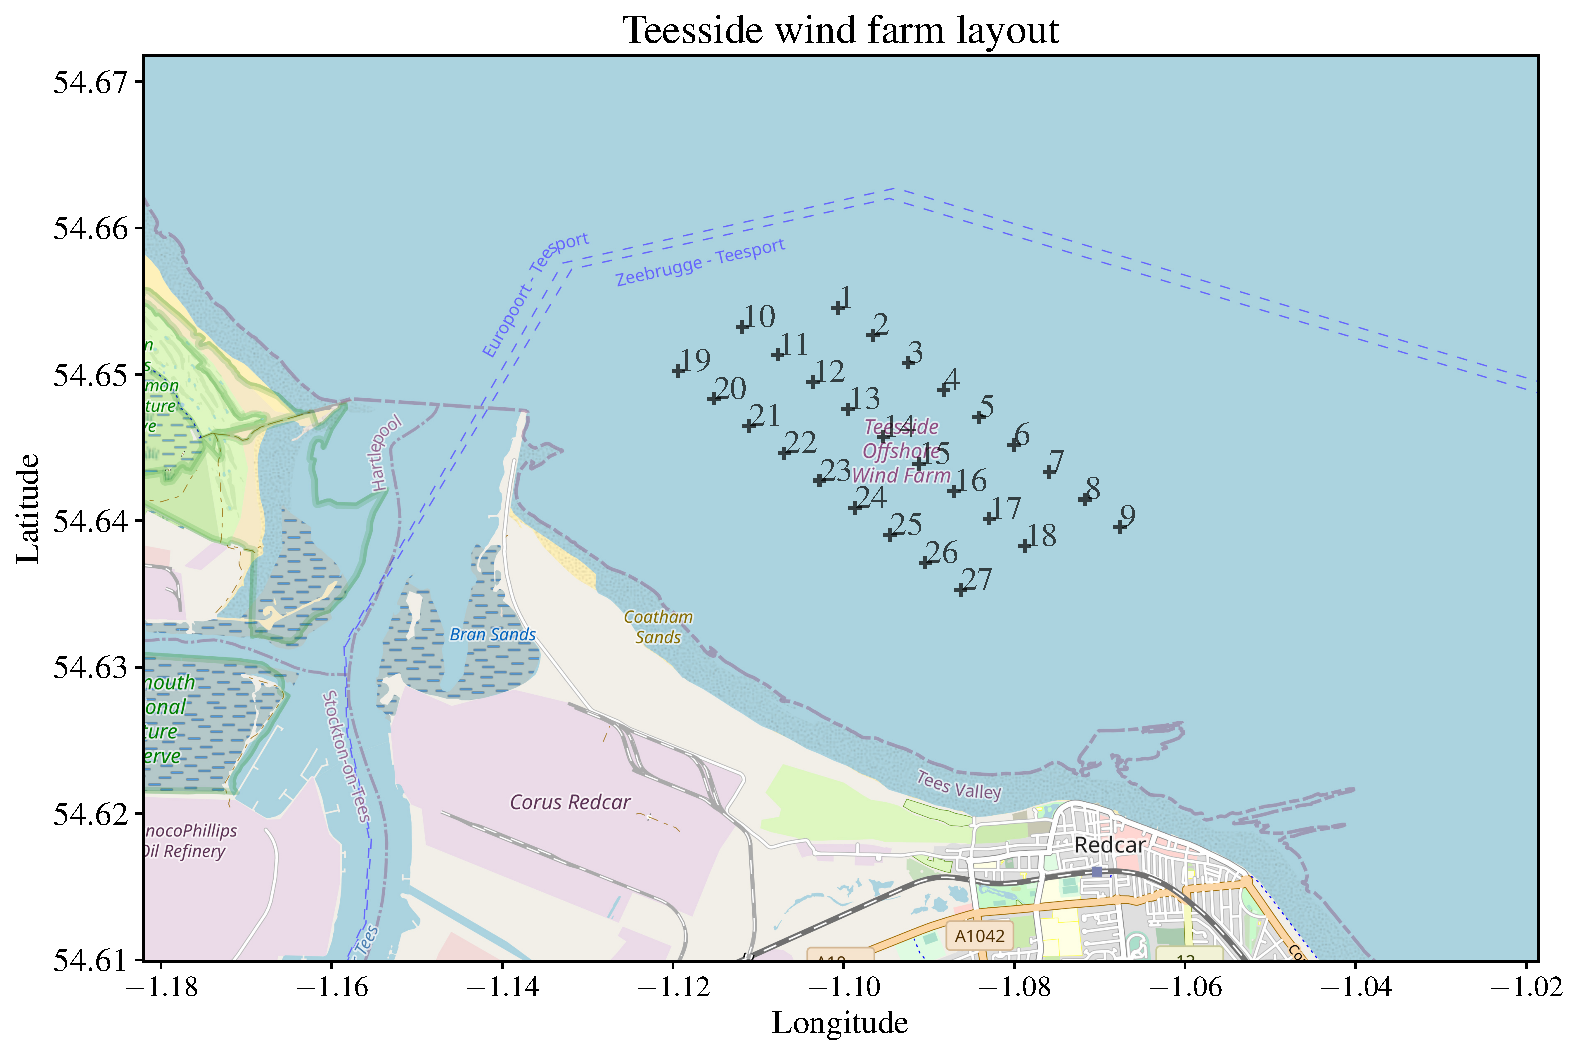
\includegraphics[width=0.6\linewidth]{part2/figures/DCE/teesside/map_teesside_layout.pdf}
    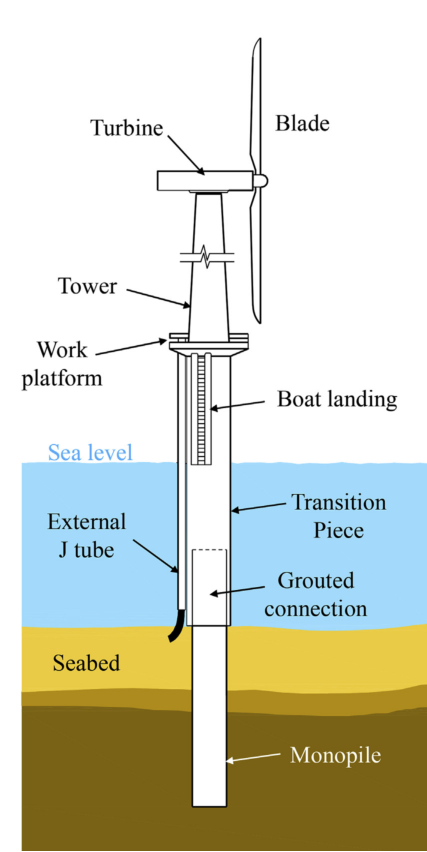
\includegraphics[width=0.25\linewidth]{part2/figures/DCE/teesside/owt_diagram.pdf}
\end{center}
\caption{Teesside wind farm layout (left). Monopile OWT diagram \citep{chen_2018_owt_diagram} (right).}
\label{fig:teesside_layout}
\end{figure}

%------------------------------------------------------------%
\subsection{Measured environmental data}
%------------------------------------------------------------%
During the lifespan of a wind farm project, environmental data is collected at different phases. 
In order to decide on the construction of a wind farm, meteorological masts, and wave buoys are usually installed on a potential site for a few years. 
After its construction, each wind turbine is equipped with monitoring instruments (e.g., cup anemometers). 
In total, five years of wind data have been collected on the turbines which are not affected by the wake on this site. 
Their acquisition system (usually called ``SCADA'' for ``Supervisory Control And Data Acquisition'') has a sampling period of ten minutes. 
The wave data arise from a buoy placed in the middle of the farm. 
These data describe the physical features listed in Table \ref{tab:envi_variables_c4}. 
A limitation of the present study is that its controller-induced uncertainty (like wind misalignment) is not considered. 

\begin{table*} 
    \begin{center}
    \begin{tabularx}{\textwidth}{@{\extracolsep\fill}llll@{}}
    \hline
    Variable & Notation & Unit & Description\\
    \hline
    Mean wind speed & $U$ & $\mathrm{m.s^{-1}}$ & 10-min. average horizontal wind speed\\
    Wind turbulence & $\sigma_U $ & $\mathrm{m.s^{-1}}$ & 10-min. wind speed standard deviation\\
    Wind direction\footnotemark & $\theta_{\mathrm{wind}} $ & deg. &  10-min. average wind direction\\
    Significant wave height & $H_s $ & m & Significant wave height\\
    Peak wave period & $T_p $  & $\mathrm{s}$ & Peak 1-hour spectral wave period \\
    Wave direction & $\theta_{\mathrm{wave}} $ & deg. &  10-min. average wave direction\\
    \hline
    \end{tabularx}
    \caption{Description of the environmental data.}
    \label{tab:envi_variables_c4}
    \end{center}
\end{table*}

\footnotetext{Note that the two directional variables could be replaced by a wind-wave misalignment variable for a bottom-fixed technology, however, our framework can be directly transposed to floating models.}

The Teesside farm is located close to the coast, making the environmental conditions very different depending on the direction (see the wind farm layout in \fig{fig:teesside_layout}). 
Since measures are also subject to uncertainties, a few checks were made to ensure that the data were physically consistent. 
Truncation bounds were applied since this study is focused on central tendency estimation (i.e., mean behavior) rather than extreme values. 
In practice, this truncation only removes extreme data points (associated with storm events). 
In addition, a simple trigonometric transform is applied to each directional feature to take into account their cyclic structure. 
Finally, the remaining features are rescaled (i.e., using a min-max normalization). 

Teesside's environmental data is illustrated by its copulogram in \fig{fig:envi_pairplot}, a graphical tool presented in Section~\ref{sec:copulogram} to visualize multivariate data. 
The copulogram exhibits the marginals with univariate kernel density estimation plots (in the diagonal), and the dependence structure with scatter plots in the normalized rank space (in the upper triangle). 
Looking at data in the rank space instead of the initial space allows one to observe the ordinal associations between variables. 
The scatter plots of normalized ranks are actually a representation of the empirical copula density.
Two independent variables will present a uniformly distributed scatter plot in the rank space. 
In the lower triangular matrix, the scatter plots are set in the physical space, merging the effects of the marginals and the dependencies (as in the usual visualization offered by the matrix plot). 
Since the dependence structure is theoretically modeled by an underlying copula, this plot is called \emph{copulogram}, generalizing the well-known ``correlogram'' to nonlinear dependencies. 
It gives a synthetic and empirical decomposition of the dataset that was implemented in a new open source Python package named \texttt{\href{https://github.com/efekhari27/copulogram}{copulogram}}\footnote{GitHub repository: \url{https://github.com/efekhari27/copulogram}}.

\begin{figure}[!h]
    \begin{center}
        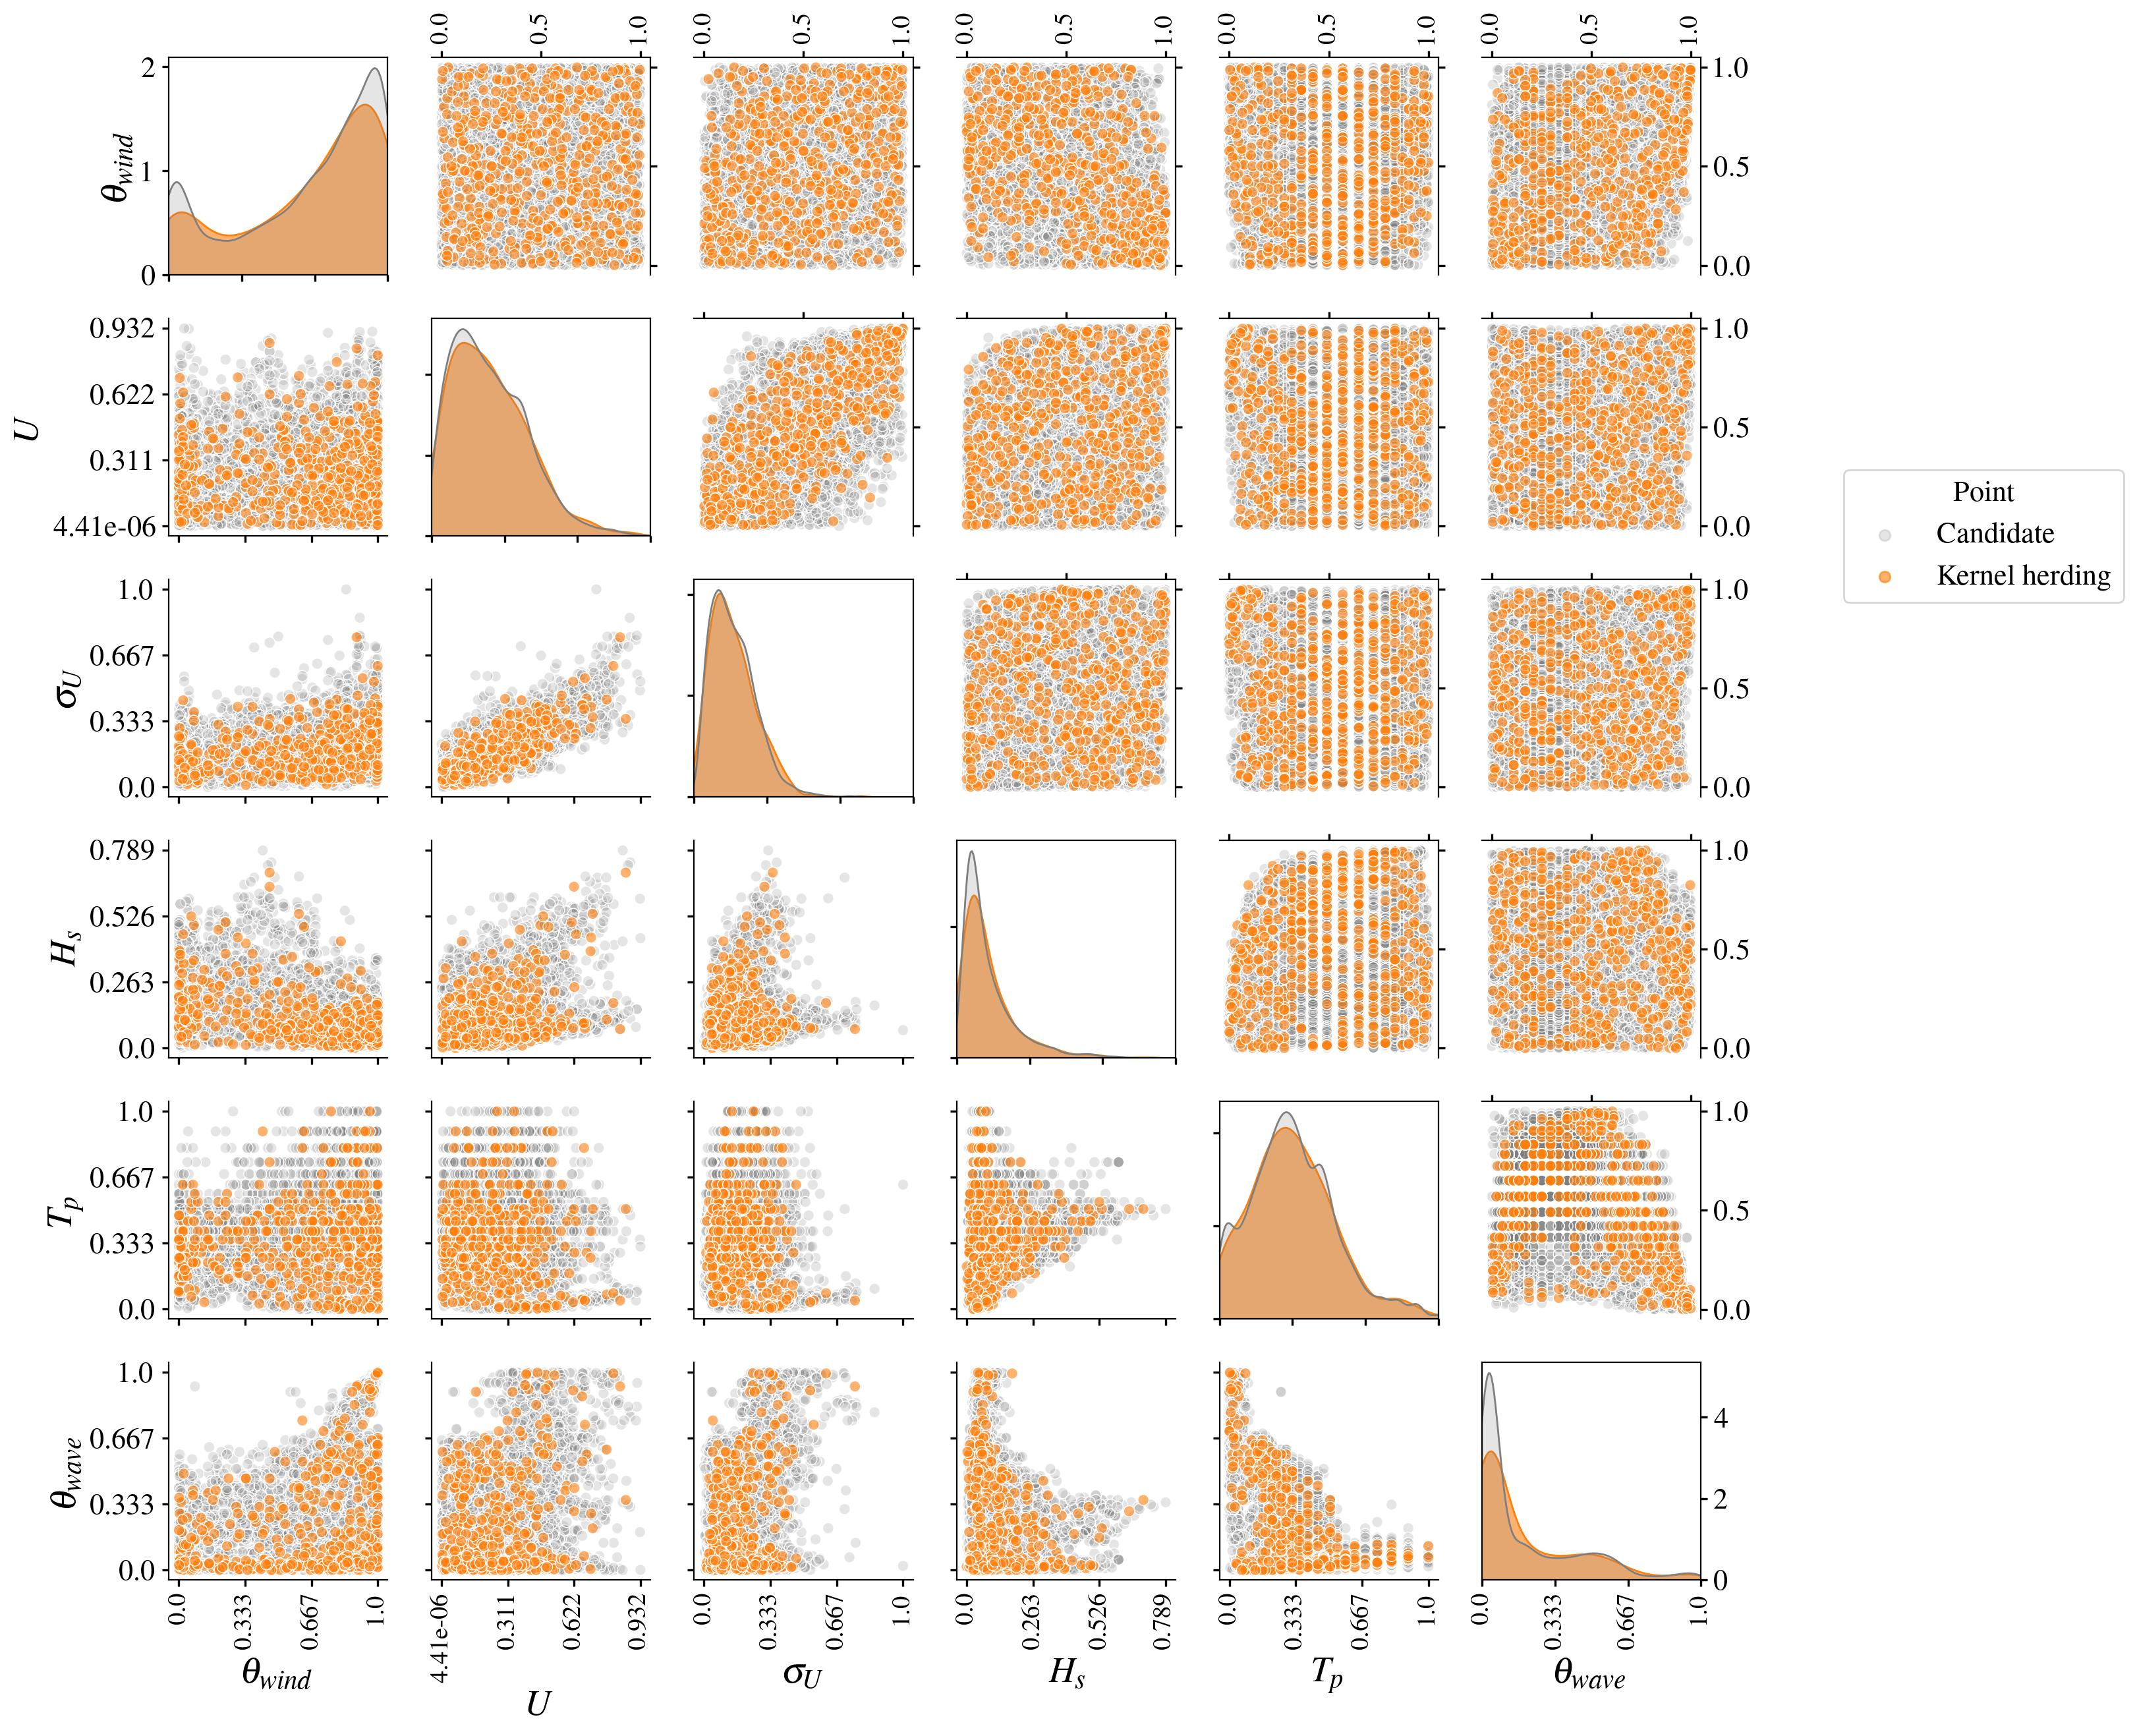
\includegraphics[width=\linewidth]{part2/figures/DCE/teesside/pairplot_kh.jpg}    
    \end{center}
    \caption{Copulogram of the Teesside measured data ($N=10^4$ in grey), kernel herding subsample ($n=500$ in orange). 
    Marginals are represented by univariate kernel density estimation plots (diagonal), the dependence structure with scatter plots in the rank space (upper triangle). 
    Scatter plots on the bottom triangle are set in the physical space.}
    \label{fig:envi_pairplot}
\end{figure}

On \fig{fig:envi_pairplot}, a large sample $\iS \subset \iD_{\bX}$ (with size $N=10^4$) is randomly drawn from the entire Teesside data (with size $N_{\mathrm{Teesside}} = 2\times 10^5$), and plotted in grey. 
In the same figure, the orange matrix plot is a subsample of the sample $\iS$, selected by kernel herding, a method minimizing some discrepancy measure with the sample $\iS$ that will be presented in Section~\ref{sec:sec43}. 
For this example, generating the kernel herding subsample takes under one minute, which is negligible compared with the simulation time of OWT models. 
Visually, this orange subsample seems to be representative of the original sample both in terms of marginal distributions and dependence structure. 
In the following study, the large samples $\iS$ will be considered as an empirical representation of the distribution of the random vector $\bX \in \iD_{\bX}$, with probability density function $f_{\bX}$, and called \textit{candidate set}. 
Kernel herding allows direct subsampling from this large and representative dataset, instead of fitting a joint distribution and generating samples from it.
Indeed, fitting a joint distribution would introduce an additional source of error in the uncertainty propagation process.
Note that a proper parametric model fit would be challenging for complex dependence structures such as the one plotted on \fig{fig:envi_pairplot}. 
As examples of works that followed this path, one can mention the work of \citet{li_zhan_2020} who built a parametric model of a similar multivariate distribution using vine copulas. 


For a similar purpose and to avoid some limits imposed by the parametric framework, 
a nonparametric approach coupling empirical Bernstein copula fitting with kernel density estimation of the marginals is proposed in Subsection~\ref{sec:4ebc}.


%------------------------------------------------------------%
\subsection{Non parametric fit with empirical Bernstein copula}\label{sec:4ebc}
%------------------------------------------------------------%
Instead of directly subsampling from a dataset such as the one from \fig{fig:envi_pairplot}, one could first infer a multivariate distribution and generate a sample from it. 
However, accurately fitting such complex multivariate distributions is challenging. 
The amount of available data is large enough to make nonparametric inference a viable option.

The Sklar theorem \citep{durante_2015_copula} states that the multivariate distribution of any random vector $\mathbf{X} \in \R^d, d \in \N^*$ can be broken down into two objects:
\begin{enumerate}
    \item A set of univariate marginal distributions to describe the behavior of the individual variables;
    \item A function describing the dependence structure between all variables, called a \textit{copula}.
\end{enumerate}
This theorem states that considering a random vector $\mathbf{X} \in \R^d$, with its cumulative distribution function $F$ and its marginals $\{F_i\}_{i=1}^d$, there exists a copula $C: [0, 1]^d \rightarrow [0, 1]$, such that:
\begin{equation}
    F(x_1, \dots, x_d) = C\left(F_1(x_1), \dots, F_d(x_d)\right). 
\end{equation}

It allows us to divide the problem of fitting a joint distribution into two independent problems: fitting the marginals and fitting the copula. 
The empirical Bernstein copula is a nonparametric copula approximation method introduced and applied to similar data in Chapter~\ref{chpt:3}. 
Provided a large enough learning set $\bX_n$ (over five years in the present case), the EBC combined with kernel density estimation for the marginals fits well the environmental joint distribution related to the dataset in \fig{fig:envi_pairplot}. 
Moreover, the densities of the EBC are available in an explicit form, making Monte Carlo or quasi-Monte Carlo generation easy. 
As discussed in Chapter~\ref{chpt:3}, this method is sensitive to the chosen polynomial orders $\{m_j\}_{j=1}^d$ and the learning set size. 


%------------------------------------------------------------%
\subsection{Fatigue assessment}
%------------------------------------------------------------%
As described in \fig{fig:bloc_diagram}, a typical DIEGO simulation returns a 10-minute multiaxial stress time series at each node $i \in \N$ of the 1D meshed structure. 
Since classical fatigue laws are established for uniaxial stresses, the first step is to compute one equivalent Von Mises stress time series at each structural node.
The present section recalls the main concepts but fatigue assessment is further discussed in Subsection~\ref{sec:235}. 

The foundation and the tower of an OWT are a succession of tubes with various sections connected by bolted or welded joints. 
Our work focuses on the welded joints at the mudline level, identified as a critical area for the structure. 
This hypothesis is confirmed in the literature by different contributions, see e.g., the results of \citet{muller_cheng_2018} in Figure 12, or \citet{katsikogiannis_2021_owt_fatigue}. 
At the top of the turbine, the fatigue is commonly studied at the blade root, which was not studied here since the blades in composite material have different properties (see e.g., \citealp{dimitrov_2013}). 
Note that the OWT simulations provide outputs allowing us to similarly study any node along the structure (without any additional computational effort).

To compute fatigue in a welded joint, the external circle of the welding ring is discretized for a few azimuth angles $\theta \in \R_+$ (see the red points in the monopile cross-section on the right in \fig{fig:wind_wave_roses}). 
The equivalent Von Mises stress time series is then reported on the external welding ring for an azimuth $\theta$. 
According to \cite{li_zhan_2020} and our own experience, the most critical azimuth angles are roughly aligned with the main wind and wave directions (whose distributions are illustrated in \fig{fig:wind_wave_roses}). 
Looking at these illustrations, the wind and wave conditions have a very dominant orientation, which is explained by the closeness of the wind farm to the shore. 
Then, it is assumed that azimuth angles in these directions will be more solicited, leading to higher fatigue damage. 
To assess fatigue damage, rainflow counting \citep{dowling_1972} first identifies the stress cycles and their respective amplitudes (using the implementation of the ASTM E1049-85 rainflow cycle counting algorithm from the Python package \texttt{rainflow}\footnote{\href{https://github.com/iamlikeme/rainflow}{https://github.com/iamlikeme/rainflow}}). 
For each identified stress cycle of amplitude, $s \in \R_+$, the so-called ``Stress vs. Number of cycles'' curve (also called the ``S-N curve'' or ``W\"ohler curve'') allows one to estimate the number $N_{\mathrm{c}}$ of similar stress cycles necessary to reach fatigue ruin. 
The S-N curve, denoted by $W(\cdot)$ is an affine function in the log-log scale with slope $-m$ and y-intercept $a$:
\begin{equation}
    N_{\mathrm{c}}(s) = a s^{-m}, \, a\in\R_+, \, m\in\R_+.
    \label{eq:wohler}
\end{equation}

Finally, a usual approach to compute the damage is to aggregate the fatigue contribution of each stress cycle identified using Miner’s rule. 
Damage occurring during a 10-minute operating time is simulated and then scaled up to the OWT lifetime. 
More details regarding damage assessment and the W\"ohler curve used are available in \citet[Sec. 2.4.6]{dnv_fatigue_2016}. 
For a realization $\bx \in \iD_{\bX}$ of environmental conditions, at a structural node $i$, an azimuth angle $\theta$; $k \in \N$ stress cycles of respective amplitude $\{s_{i, \theta}^{(j)}(\bx)\}_{j=1}^k$ are identified. 
Then, Miner's rule (see Subsection~\ref{sec:235}) defines the damage function $g_{i, \theta}(\bx): \iD_{\bX} \rightarrow \R_+$ by:
\begin{equation}
    g_{i, \theta}(\bx) = \sum_{j=1}^{k} \frac{1}{N_{\mathrm{c}}\left(s_{i, \theta}^{(j)}(\bx)\right)}.
    \label{eq:miner1}
\end{equation}

As defined by the DNV standards for OWT fatigue design \citep{dnv_fatigue_2016}, the quantity of interest in the present chapter is the ``mean damage'' $D_{\mathrm{c}}^{i, \theta}$ (also called ``mean cumulative damage''), computed at a node $i$, for an azimuth angle $\theta$:
\begin{equation}
    D_{\mathrm{c}}^{i, \theta} = \E[g_{i, \theta}(\bX)] = \int_{\iD_\bX} g_{i, \theta}(\bx) f_{\bX}(\bx)\, \dd \bx \,.
    \label{eq:mean_integral}
\end{equation}

To get a preview of the distribution of this output random variable $g_{i, \theta}(\bX)$, a histogram of a large Monte Carlo simulation ($N_{\mathrm{ref}}=2000$) is represented in \fig{fig:histo_mc} (with a log scale). 
In this case, the log-damage histogram presents a little asymmetry but it is frequently modeled by a normal distribution (see e.g., \citealp{teixeira_2019}). 

\begin{figure}[!h]
\begin{center}
    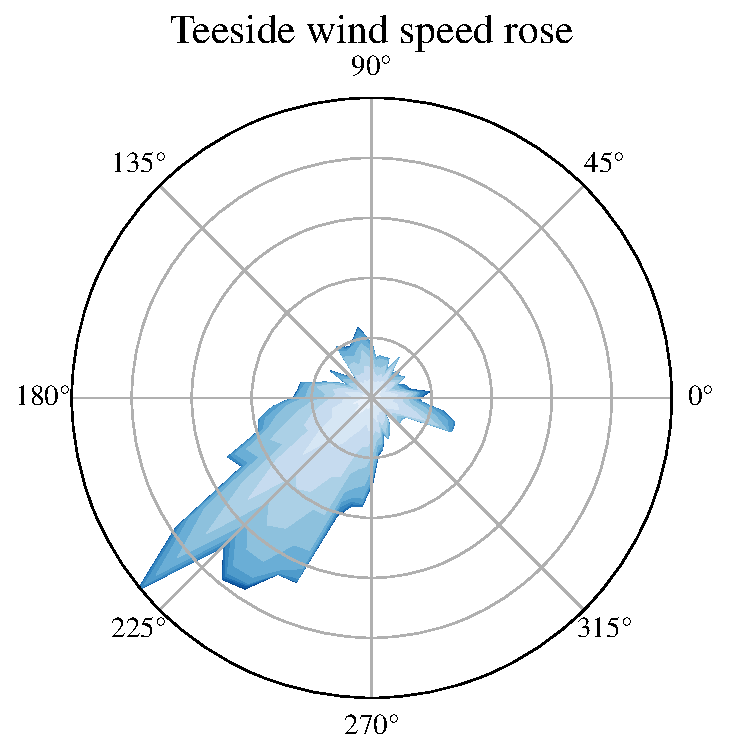
\includegraphics[width=0.3\textwidth]{part2/figures/DCE/teesside/teeside_wind_rose.pdf} \quad
    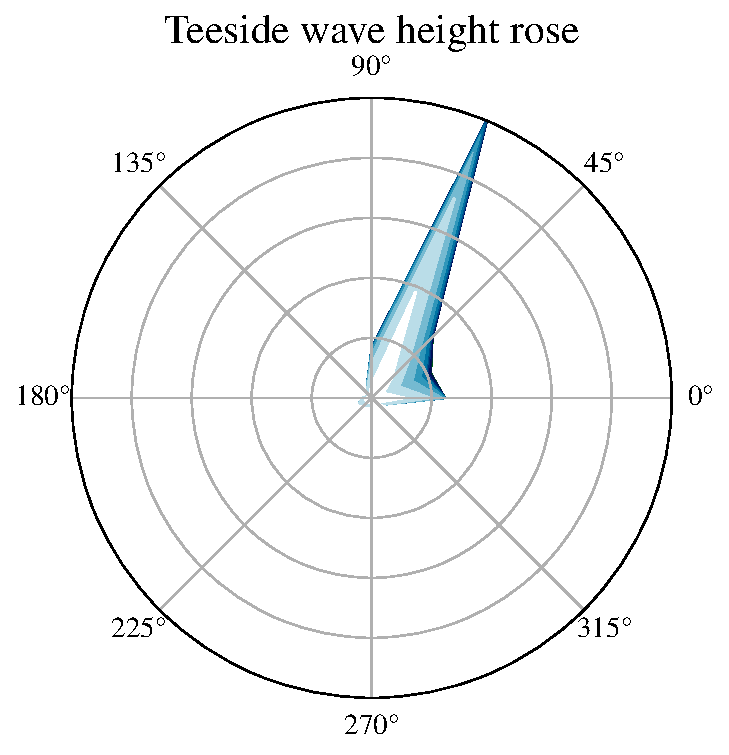
\includegraphics[width=0.3\textwidth]{part2/figures/DCE/teesside/teeside_wave_rose.pdf} \quad
    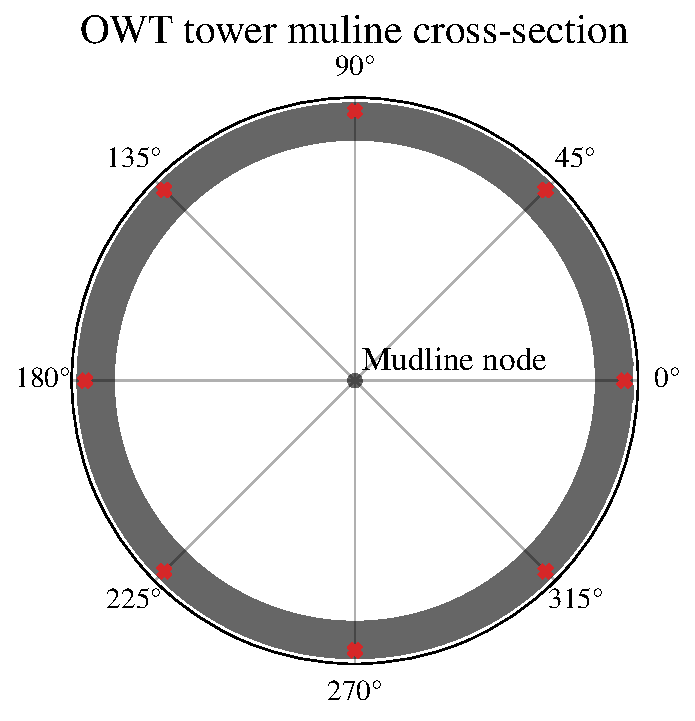
\includegraphics[width=0.3\textwidth]{part2/figures/DCE/teesside/mudline_crossection.pdf}
\end{center}
\caption{Angular distribution of the wind and waves with a horizontal cross-section of the OWT structure and the mudline. 
Red crosses represent the discretized azimuths for which the fatigue is computed.}
\label{fig:wind_wave_roses}
\end{figure}

\begin{figure}[!h]
\begin{center}
    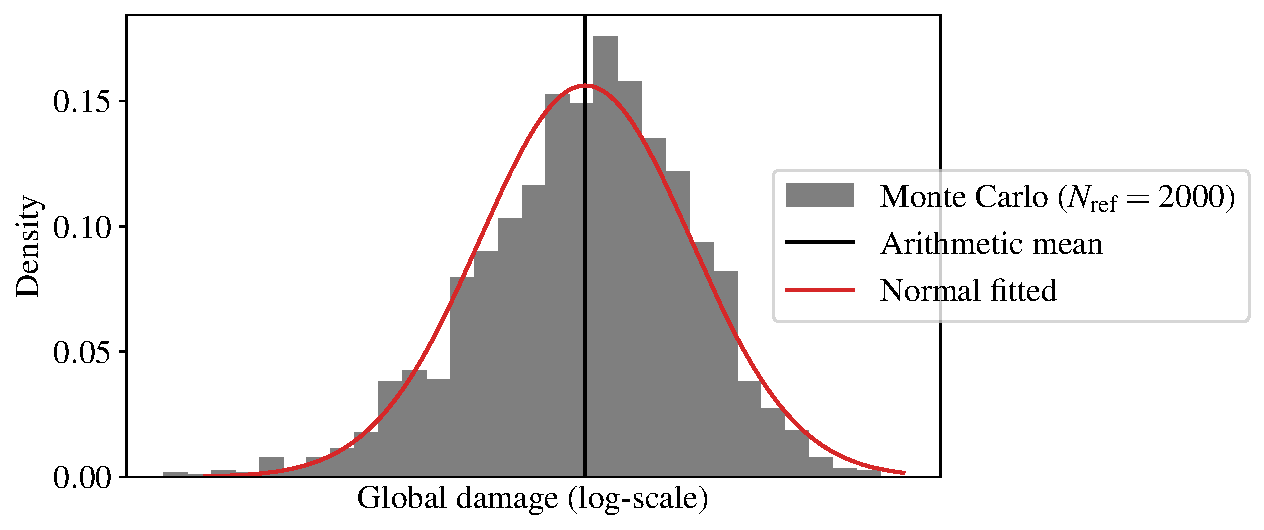
\includegraphics[width=0.7\textwidth]{part2/figures/DCE/teesside/reference_log_histogramNode1_45.pdf}
\end{center}
\caption{Histogram of the log-damage, at mudline, azimuth 45 deg. (Monte Carlo reference sample).}
\label{fig:histo_mc}
\end{figure}

%============================================================%
\section{Numerical integration procedures for mean damage estimation}\label{sec:sec43}
%============================================================%
The present section explores different methods aiming at approximating the integral of a function against a probability measure. 
In the case of OWT mean damage estimation, these methods can be used for defining efficient design load cases. 
This problem is equivalent to the central tendency estimation of $\bY = g(\bX)$, the image of the environmental random variable $\bX$ by the damage function $g(\cdot): \iD_\bX \to \R$ (see e.g., \eq{eq:mean_integral}). 
Considering a measurable space $\iD_\bX \subset \R^d, d \in \N^*$, associated with a known probability measure $\pi$, this section studies the approximation of integrals of the form $\int_{\iD_\bX} g(\bx) \dd\pi(\bx)$. 
%------------------------------------------------------------%
\subsection{Quadrature rules and quasi-Monte Carlo methods}
%------------------------------------------------------------%
Numerical integration authors may call this generic problem \emph{probabilistic integration} \citep{briol_oates_2019}. 
In practice, this quantity of interest is estimated on an $n$-sized set of damage realizations $\by_n = \left\{g(\bx^{(1)}), \dots, g(\bx^{(n)})\right\}$ of an input sample $\bX_n = \left\{\bx^{(1)}, \dots, \bx^{(n)}\right\}$. 
A weighted arithmetic mean of the realizations $\left\{g(\bx^{(1)}), \dots, g(\bx^{(n)})\right\}$ is called a \emph{quadrature rule} with a set of unconstrained weights $\bw_n = \{w_1, \dots, w_n\} \in \R^n$:
\begin{equation}
    I_{\pi}(g) = \int_{\iD_\bX} g(\bx) \dd\pi(\bx) \approx \sum_{i=1}^n w_i g(\bx^{(i)}).
    \label{eq:quadrature_rule}
\end{equation}
Our numerical experiment framework often implies that the function $g$ is costly to evaluate, making the realization number limited. 
For a given sample size $n$, our goal is to find a set of tuples $\left\{\bx^{(i)}, w_i \right\}_{i=1}^n$ (i.e., quadrature rule), giving the best approximation of our quantity. 
In the literature, a large panel of numerical integration methods has been proposed to tackle this problem. 
For example, \cite{bos_2020} recently developed a quadrature rule based on arbitrary sample sets which was applied to a similar industrial OWT use case.  

Alternatively, sampling methods rely on generating a set of points $\bX_n$ drawn from the input distribution to compute the arithmetic mean of their realizations (i.e., uniform weights $\left\{w_i = \frac1n \right\}_{i=1}^n$). 
Among them, low-discrepancy sequences, also called ``quasi-Monte Carlo'' sampling (e.g., Sobol', Halton, Faure sequences) are known to improve the standard Monte Carlo convergence rate and will be used as a deterministic reference method in the following numerical experiments \citep{leobacher_2014}.

\paragraph{Quantization of probability measures and quadrature}
%------------------------------------------------------------%
When dealing with probabilistic integration such as \eq{eq:quadrature_rule}, a quadrature rule is a finite representation of a continuous measure $\pi$ by a discrete measure $\zeta_n = \sum_{i=1}^n w_i \delta(\bx^{(i)})$ (weighted sum of Dirac distributions at the design points $\bX_n$).
In the literature, this procedure is also called \emph{quantization} of a continuous measure $\pi$. 
Overall, numerical integration is a particular case of probabilistic integration against a uniform input measure. 
For uniform measures, the Koksma-Hlawka inequality \citep{morokoff_1995} provides a useful upper bound on the absolute error of a quadrature rule: 
\begin{equation}
    \left| \int_{[0, 1]^d} g(\bx) \dd \bx - \frac1n \sum_{i=1}^n g(\bx^{(i)})\right| \leq  V(g) D_n^*(\bX_n).
    \label{eq:KH_inequality}
\end{equation}
As presented in \cite{oates_21}, $V(g) = \sum_{\mathfrak{u}\subseteq\{1, \dots, p \}} \int_{[0, 1]^\mathfrak{u}} \left| \frac{\partial^{\mathfrak{u}}g}{\partial \bx_{\mathfrak{u}}}(\bx_{\mathfrak{u}}, 1)\right| \dd\bx$, quantifies the complexity of the integrand, 
while $D_n^*(\bX_n)$ evaluates the discrepancy to uniformity of the design $\bX_n$. 
Therefore, the Koksma-Hlawka inequality shows that the quadrature rule's accuracy relies on the good quantization of $\pi$ by $\bX_n$. 
For a uniform measure $\pi$, the star discrepancy $D_n^*(\bX_n)$ is a metric assessing how far from uniformity a sample $\bX_n$ is. 
When generalizing to a non-uniform measure, a good quantization of $\pi$ should also lead to a good approximation of the quantity. 


%------------------------------------------------------------%
\subsection{Kernel herding sampling}\label{sec:4khsubsec}
%------------------------------------------------------------%

Quasi-Monte Carlo sampling methods widely rely on a metric of uniformity, called \textit{discrepancy}. 
To go beyond uniform measures, Appendix~\ref{apx:B} introduces a kernel-based discrepancy, generalizing the discrepancy concept to non-uniform measures. 
This tool, named the maximum mean discrepancy (MMD) allows comparing multivariate distributions by embedding them in a specific function space. 
In this manuscript, the MMD was employed as a tool for statistical testing and quantifying the perturbations of distributions in Chapter~\ref{chpt:3}, and for sensitivity analysis in Section~\ref{sec:gsa}.

Herin, the MMD is used to build a quadrature rule by sampling from a known measure. 
In other words, to quantize a known target measure $\pi$ by a design sample $\bX_n$. 
For practical reasons, the design construction is done sequentially. 
Sequential strategies have also been used to learn and validate regression models for statistical learning (see \citealp{fekhari_iooss_2023}). 
Moreover, since each realization is supposed to be obtained at the same unitary cost, the quadrature weights are first fixed as uniform during the construction of the design $\bX_n$.

\emph{Kernel herding} (\abv{kh}), proposed by \cite{chen_welling_2010}, is a sampling method that offers a quantization of the measure $\pi$ by minimizing a squared MMD when adding points iteratively. 
With a current design $\bX_n$ and its corresponding discrete distribution with uniform weights $\zeta_n= \frac{1}{n} \sum_{i=1}^{n} \delta(\bx^{(i)})$, a KH iteration is as an optimization of the following criterion, selecting the point $\bx^{(n+1)} \in \iD_{\bX}$:
\begin{align}
   \bx^{(n+1)} \in \argmin_{\bx \in \iD_{\bX}} \left\{\MMD\left(\pi, \frac{1}{n+1} \left(\delta(\bx) + \sum_{i=1}^{n} \delta(\bx^{(i)})\right)\right)^2\right\}.
   % = \argmin_{\bx \in \iD_{\bX}} \MMD\left(\pi, \frac{1}{n+1} \left(n \zeta_n  + \delta(\bx)\right)\right)
   \label{eq:mmd_criterion}
\end{align}

In the literature, two formulations of this optimization problem can be found. 
The first one uses the Frank-Wolfe algorithm (or ``conditional gradient algorithm'') to compute a linearization of the problem under the convexity hypothesis (see \citealp{lacoste_2015} and \citealp{briol_2015} for more details). 
The second one is a straightforward greedy optimization. Due to the combinatorial complexity, the greedy formulation is tractable for sequential construction only. 
Let us develop the MMD criterion from \eq{eq:mmd_design}:
\begin{subequations}
\begin{align}
    \MMD\left(\pi, \frac{1}{n+1} \left(\delta(\bx) + \sum_{i=1}^{n} \delta(\bx^{(i)})\right)\right)^2
    &= \varepsilon_\pi - \frac{2}{n+1} \sum_{i=1}^{n+1} P_{\pi}\left(\bx^{(i)}\right) + \frac{1}{(n+1)^2} \sum_{i,j=1}^{n+1} k\left(\bx^{(i)}, \bx^{(j)}\right)\\
    &= \varepsilon_\pi - \frac{2}{n+1} \left(P_\pi(\bx) + \sum_{i=1}^n P_{\pi}\left(\bx^{(i)}\right)\right)\\ &+ \frac{1}{(n+1)^2} \left(\sum_{i,j=1}^n k\left(\bx^{(i)}, \bx^{(j)}\right) + 2\sum_{i=1}^n k\left(\bx^{(i)}, \bx\right) - k(\bx, \bx) \right).
\end{align}
\end{subequations}
In the previously developed expression, only a few terms actually depend on the next optimal point $\bx^{(n+1)}$ since the target energy, denoted by $\varepsilon_\pi$, and $k(\bx, \bx)=\sigma^2$ are constant (by taking a stationary kernel). 
Therefore, the greedy minimization of the MMD can be equivalently written as: 
\begin{equation}
    \bx^{(n+1)} \in \argmin_{\bx \in \iD_{\bX}} \left\{ \frac{1}{n+1} \sum_{i=1}^n k\left(\bx^{(i)}, \bx\right) - P_\pi(\bx) \right\} = \argmin_{\bx \in \iD_{\bX}} \left\{ \frac{n}{n+1} P_{\zeta_n}(\bx) - P_{\pi}(\bx)\right\}.
    \label{eq:greedy_formulation}
\end{equation}

\medskip
\begin{remark}
For the sequential and uniformly weighted case, the formulation in \eq{eq:greedy_formulation} is almost similar to the Frank-Wolfe formulation. 
Our numerical experiments showed that these two versions generate very close designs, especially as $n$ becomes large. 
\cite{pronzato_rendas_2021} express the Frank-Wolfe formulation in the sequential and uniformly weighted case as follows:
\begin{align}
   \bx^{(n+1)} \in \argmin_{\bx \in \iD_{\bX}} \left\{P_{\zeta_n}(\bx) - P_{\pi}(\bx)\right\}.
   \label{eq:kh_criterion}
\end{align}
\end{remark}
\smallskip

\begin{remark}
In practice, the optimization problem is solved by a brute-force approach on a fairly dense finite subset $\iS\subseteq\iD_{\bX}$ of candidate points with size $N \gg n$ that emulates the target distribution, also called the ``candidate set''. 
This sample is also used to estimate the target potential $P_\pi(\bx) \approx \frac1N \sum_{i=1}^N k\left(\bx^{(i)}, \bx\right)$.
\end{remark}
\medskip

The diagram illustrated in \fig{fig:kh_algo} summarizes the main steps of a kernel herding sampling algorithm. 
One can notice that the initialization can either be done using a median point (maximizing the target potential) or from any existing design of experiments. 
This second configuration is practical when the analyst must include some characteristic points in the design (e.g., points with a physical interpretation). 

\begin{figure}
    \centering
    \begin{tikzpicture}
		\node [style=rect] (0) at (-27, 0) {Candidate set \\$\mathcal{S} \sim \pi$ ($N$-sized)};
		\node [style=rect] (1) at (-24, 0) {Covariance matrix $\mathbf{K}_N$};
		\node [style=rect] (2) at (-21, 0) {Target potential $P_\pi(\textbf{x}), \textbf{x} \in \mathcal{S}$};
		\node [style=rect] (3) at (-18, 0) {Design of experiments $\mathbf{X}_n$};
		\node [style=rect] (4) at (-15, 0) {Current potential $P_{\zeta_n}(\textbf{x}), x \in \mathcal{S}$};
		\node [style={diag_rect}] (6) at (-25, 1.1) {Discretize a \\kernel $k$ over $\mathcal{S}$};
		\node [style={diag_rect}] (7) at (-22, 1.1) {Average $\mathbf{K}_N$ \\over all the rows};
		\node [style={diag_rect}] (8) at (-19, 1.1) {Initialize \\the design $\mathbf{X}_n$ };
		\node [style={diag_rect}] (9) at (-16, 1.1) {Average $\mathbf{K}_N$\\over the $\mathbf{X}_n$ rows};
		\node [style=dot] (10) at (-25.6, 0) {};
		\node [style=dot] (11) at (-22.6, 0) {};
		\node [style=dot] (12) at (-19.6, 0) {};
		\node [style=dot] (13) at (-16.6, 0) {};
		\node (14) at (-16, -1.4) {};
		\node (15) at (-17, -1.4) {};
		\node [style=texte] (16) at (-16.5, -1.) {Add a point to $\mathbf{X}_n$ \\using \eq{eq:kh_criterion}};
		\node [style=dot] (17) at (-16.6, -1.4) {};
		\draw [style=arrow] (0) to (1);
		\draw [style=arrow] (1) to (2);
		\draw [style=arrow] (2) to (3);
		\draw [style=arrow] (3) to (4);
		\draw [style=arrow, in=-90, out=-180] (15.center) to (3);
		\draw [style=line] (15.center) to (14.center);
		\draw [style=line, in=-90, out=0] (14.center) to (4);
\end{tikzpicture}
    \caption{Greedy kernel herding algorithm.}
    \label{fig:kh_algo}
\end{figure}

As explained previously, choosing the kernel defines the function space on which the worst-case function is found (see \eq{eq:mmd_c4}). 
Therefore, this sampling method is sensitive to the kernel's choice. 
A kernel is defined, both by the choice of its parametric family (e.g., Matérn, squared exponential) and the choice of its tuning. 
The so-called ``support points'' method developed by \cite{mak_joseph_2018} is a special case of kernel herding that uses the characteristic and parameter-free ``energy-distance'' kernel (introduced by \citealp{szekely_rizzo_2013}). 
In the following numerical experiments, the energy-distance kernel will be compared with an isotropic tensor product of a Matérn kernel (with regularity parameter $\nu = 5/2$ and correlation lengths $\theta_i$), or a squared exponential kernel (with correlation lengths $\theta_i$) defined in Table \ref{tab:kernels}. 
Since the Matérn and squared exponential kernels are widely used for Gaussian process regression \citep{rasmussen_2006}, they were naturally picked to challenge the energy-distance kernel. 
The correlation lengths for the squared exponential and Matérn kernels are set using the heuristic given in \cite{fekhari_iooss_2023}, $\theta_i = n^{-1/d}, i \in \{1, \dots, d\}$. 

\begin{table*}
    \begin{center}
    \begin{tabular*}{\textwidth}{@{\extracolsep\fill}lll@{}}
    \hline
    Energy-distance & $k_E(\bx,\bx') = \frac12\, \left(\| \bx \| + \| \bx' \| - \| \bx-\bx' \|\right)$ & \\
    Squared exponential & $k_G(\bx,\bx') = \prod_{i=1}^{p} k_{\theta_{i}}(x_{i}-x'_i)$ & $k_{\theta}(x-x') = \exp \left(- \frac{(x-x')^2}{2\theta^2}\right)$\\
    Matérn $(\nu = 5/2)$ & $k_M(\bx,\bx') = \prod_{i=1}^{p} k_{5/2,\theta_{i}}(x_{i}-x'_i)$
     & $k_{5/2,\theta}(x-x') = \Bigl(1 + \frac{\sqrt{5}}{\theta} |x - x'|$ \\ 
     & & $\quad + \frac{5}{3 \theta^2} (x - x')^2 \Bigr) \exp \left( - \frac{\sqrt{5}}{\theta} |x - x'| \right)$ \\
    \hline
    \end{tabular*}
    \caption{Kernels considered in the following numerical experiments.}
    \label{tab:kernels}
    \end{center}
\end{table*}

\fig{fig:kernels} represents the covariance structure of the three kernels. 
One can notice that the squared exponential and Matérn $\nu = 5/2$ kernels are closer to one another than they are to the energy-distance. 
In fact, as $\nu$ tends to infinity, the Matérn kernel tends toward the squared exponential kernel (which has infinitely differentiable sample paths, see \citealp{rasmussen_2006}). 
For these two stationary kernels, the correlation length controls how fast the correlation between two points decreases as their distance from one another increases. 

Meanwhile, the energy distance is not stationary (but still positive and semi-definite). 
Therefore, its value does not only depend on the distance between two points but also on the norm of each of the points.
Interestingly, the energy-distance kernel is almost similar to the kernel used by \citet{hickernell_1998} to define a widely-used space-filling metric called the centered $L^2$-discrepancy. 
A presentation of these kernel-based discrepancies from the design of experiment point of view is also provided in Chapter Two from \citet{fang_liu_2018}.  

\begin{figure}[!h]
\begin{center}
    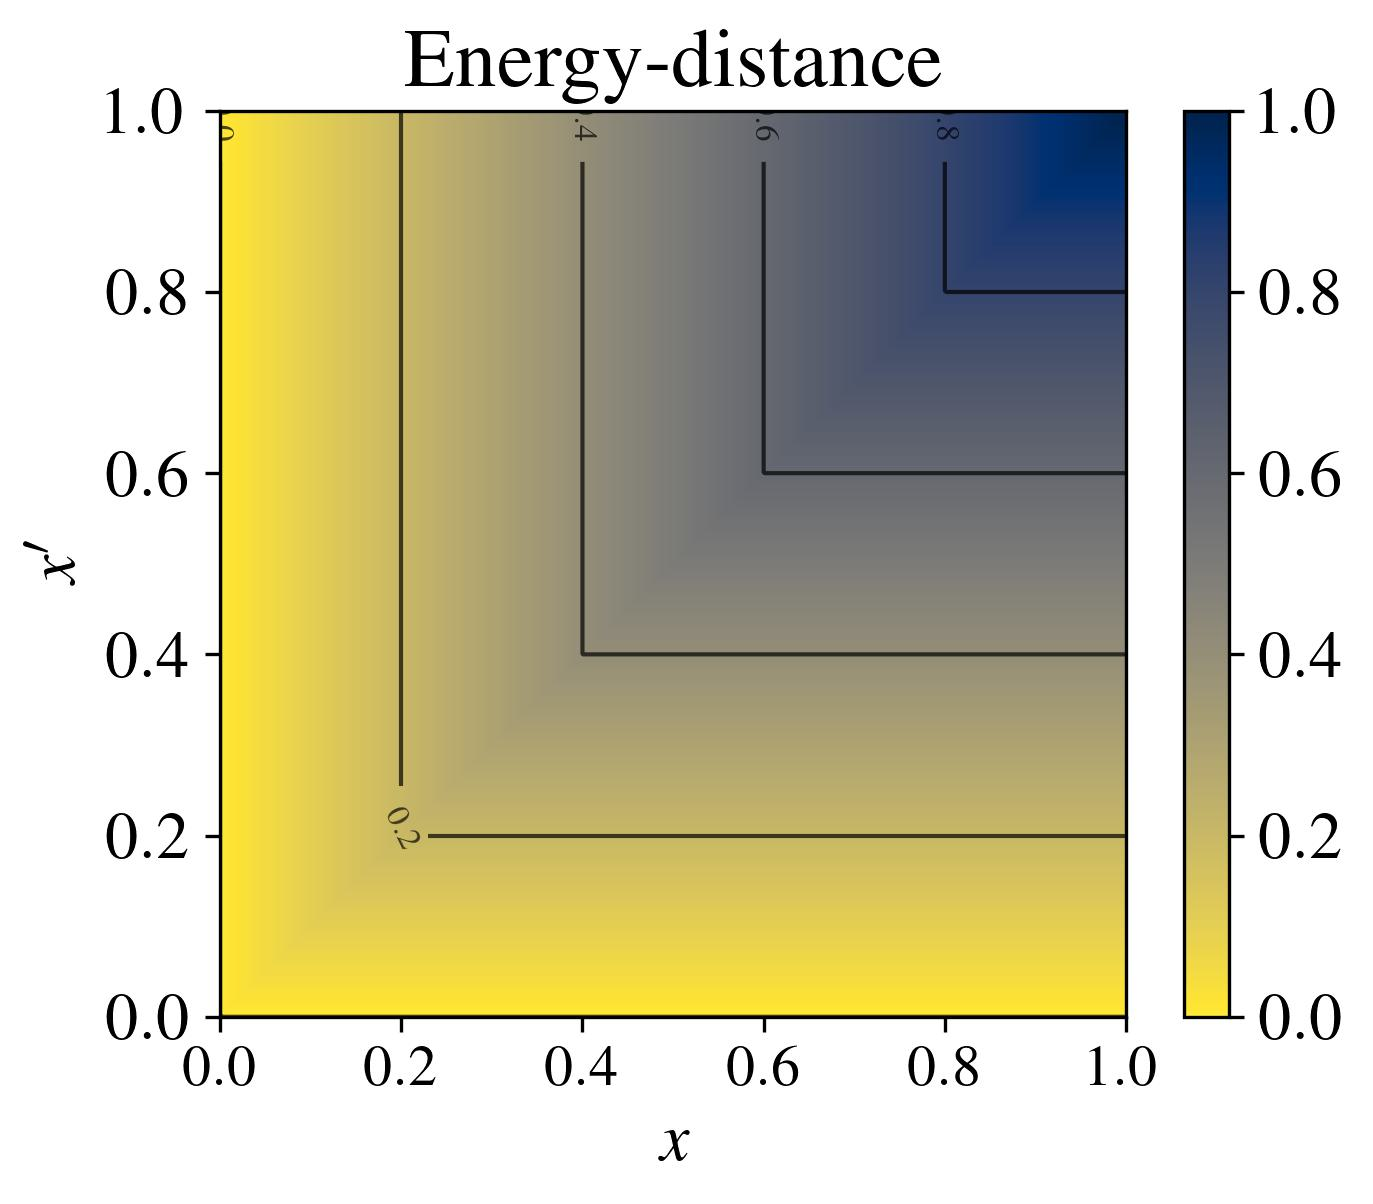
\includegraphics[width=0.32\textwidth]{part2/figures/DCE/numerical_experiments/energy_kernel.jpg}
    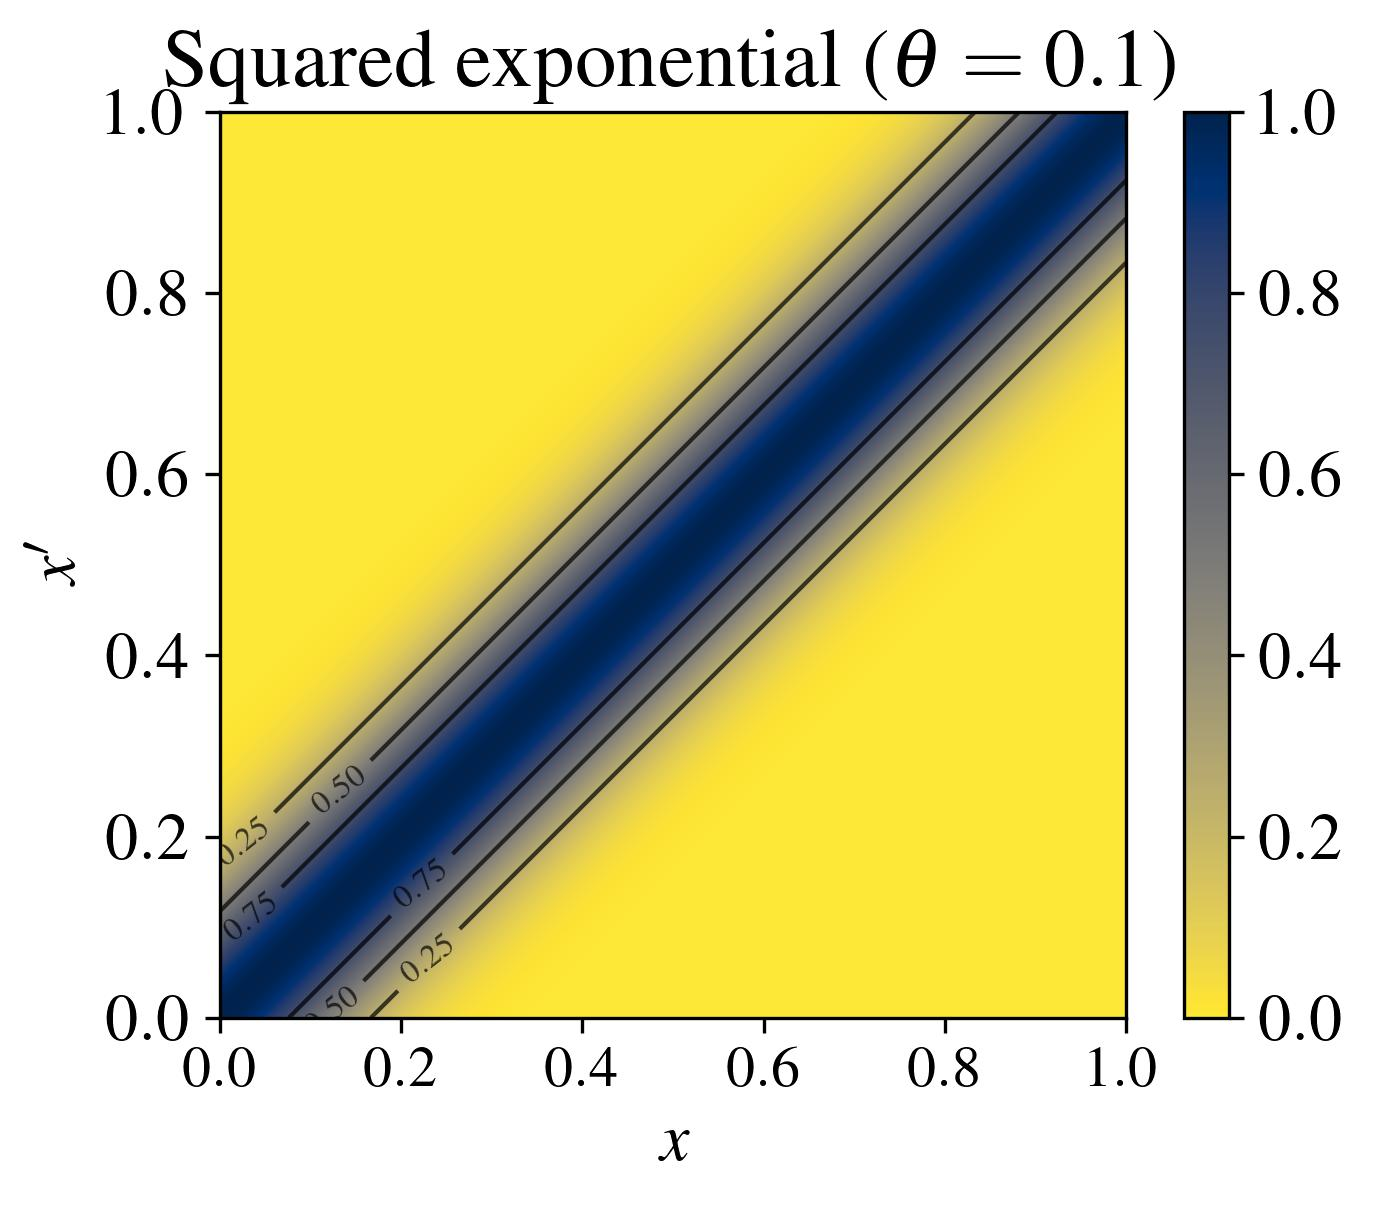
\includegraphics[width=0.32\textwidth]{part2/figures/DCE/numerical_experiments/gaussian_kernel.jpg}
    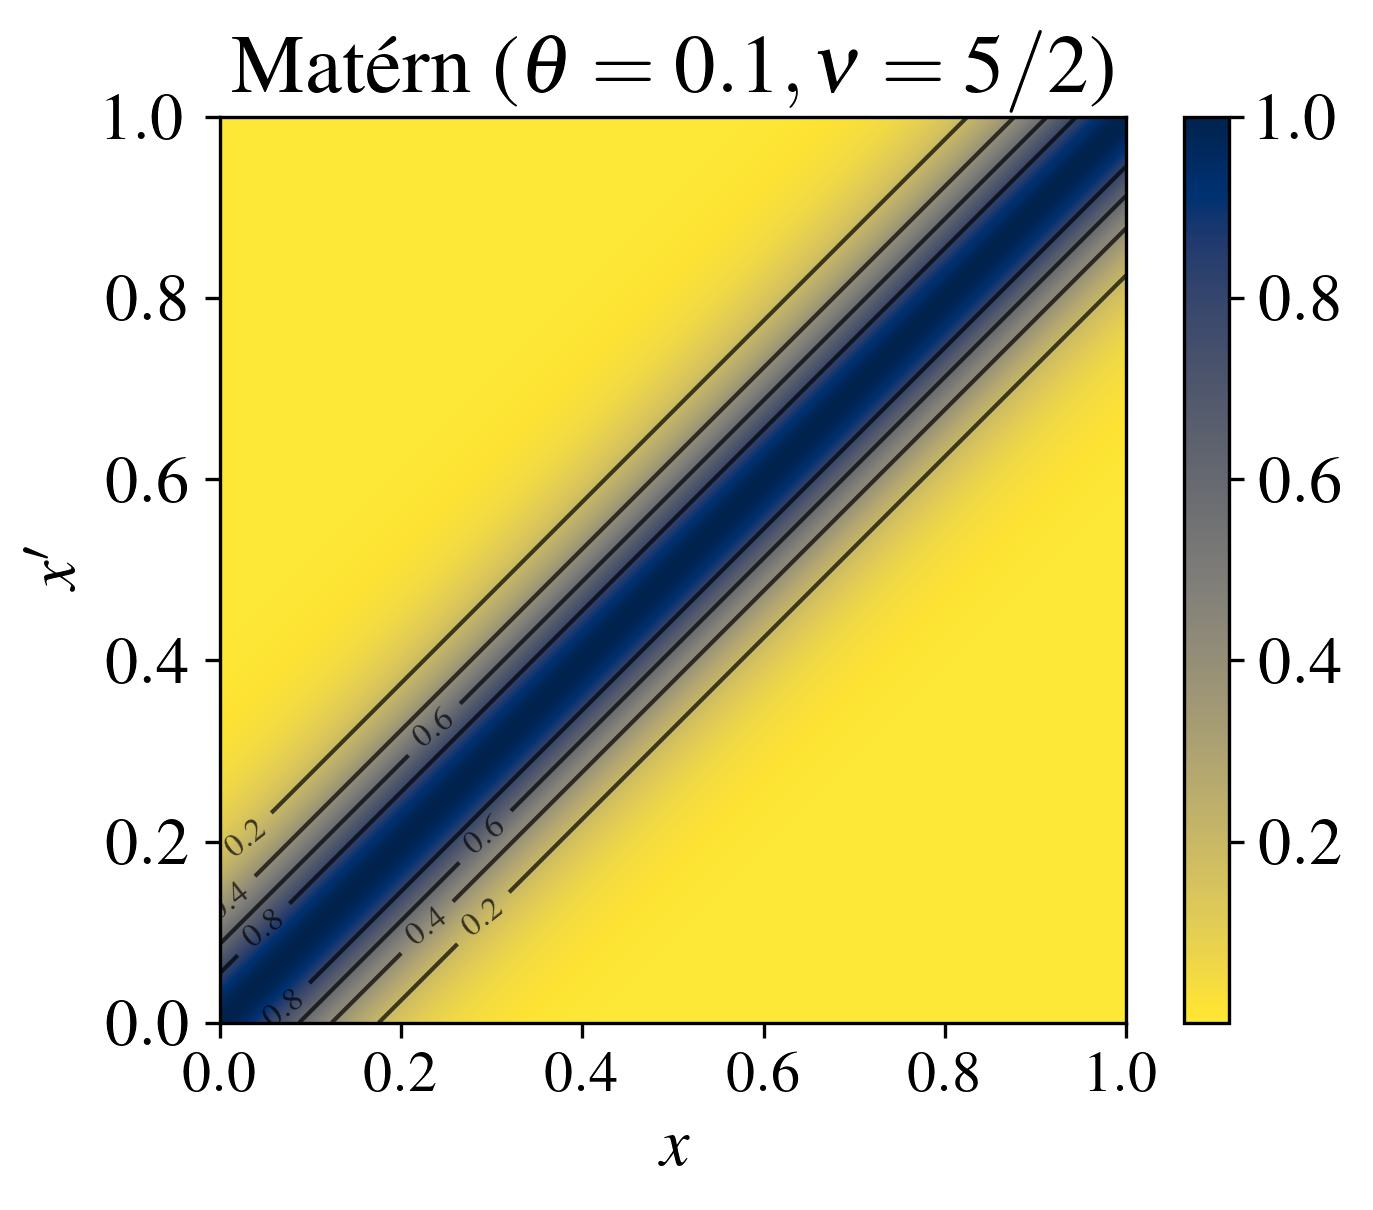
\includegraphics[width=0.32\textwidth]{part2/figures/DCE/numerical_experiments/matern_kernel.jpg}
\end{center}
\caption{Kernel illustrations (left to right: energy-distance, squared exponential, and Matérn $5/2$).} \label{fig:kernels}
\end{figure}

To illustrate the kernel herding sampling of a complex distribution, \fig{fig:KH_mixture} shows three nested samples (orange crosses for different sizes $n\in\{10, 20, 40\}$) of a mixture of Gaussian distributions with complex nonlinear dependencies (with density represented by the black isoprobability contours). 
In this example, the method seems to build a parsimonious design between each mode of the distribution (by subsampling directly without any transformation). 
The candidate set (in light grey) was generated by a large quasi-Monte sample of the underlying Gaussian mixture. 
In this two-dimensional case, this candidate set is sufficient to estimate the target potential $P_{\pi}$. 
However, the main bottleneck of kernel herding is the estimation of the potentials, which becomes costly in high dimensions.

\begin{figure}[!h]
\begin{center}
    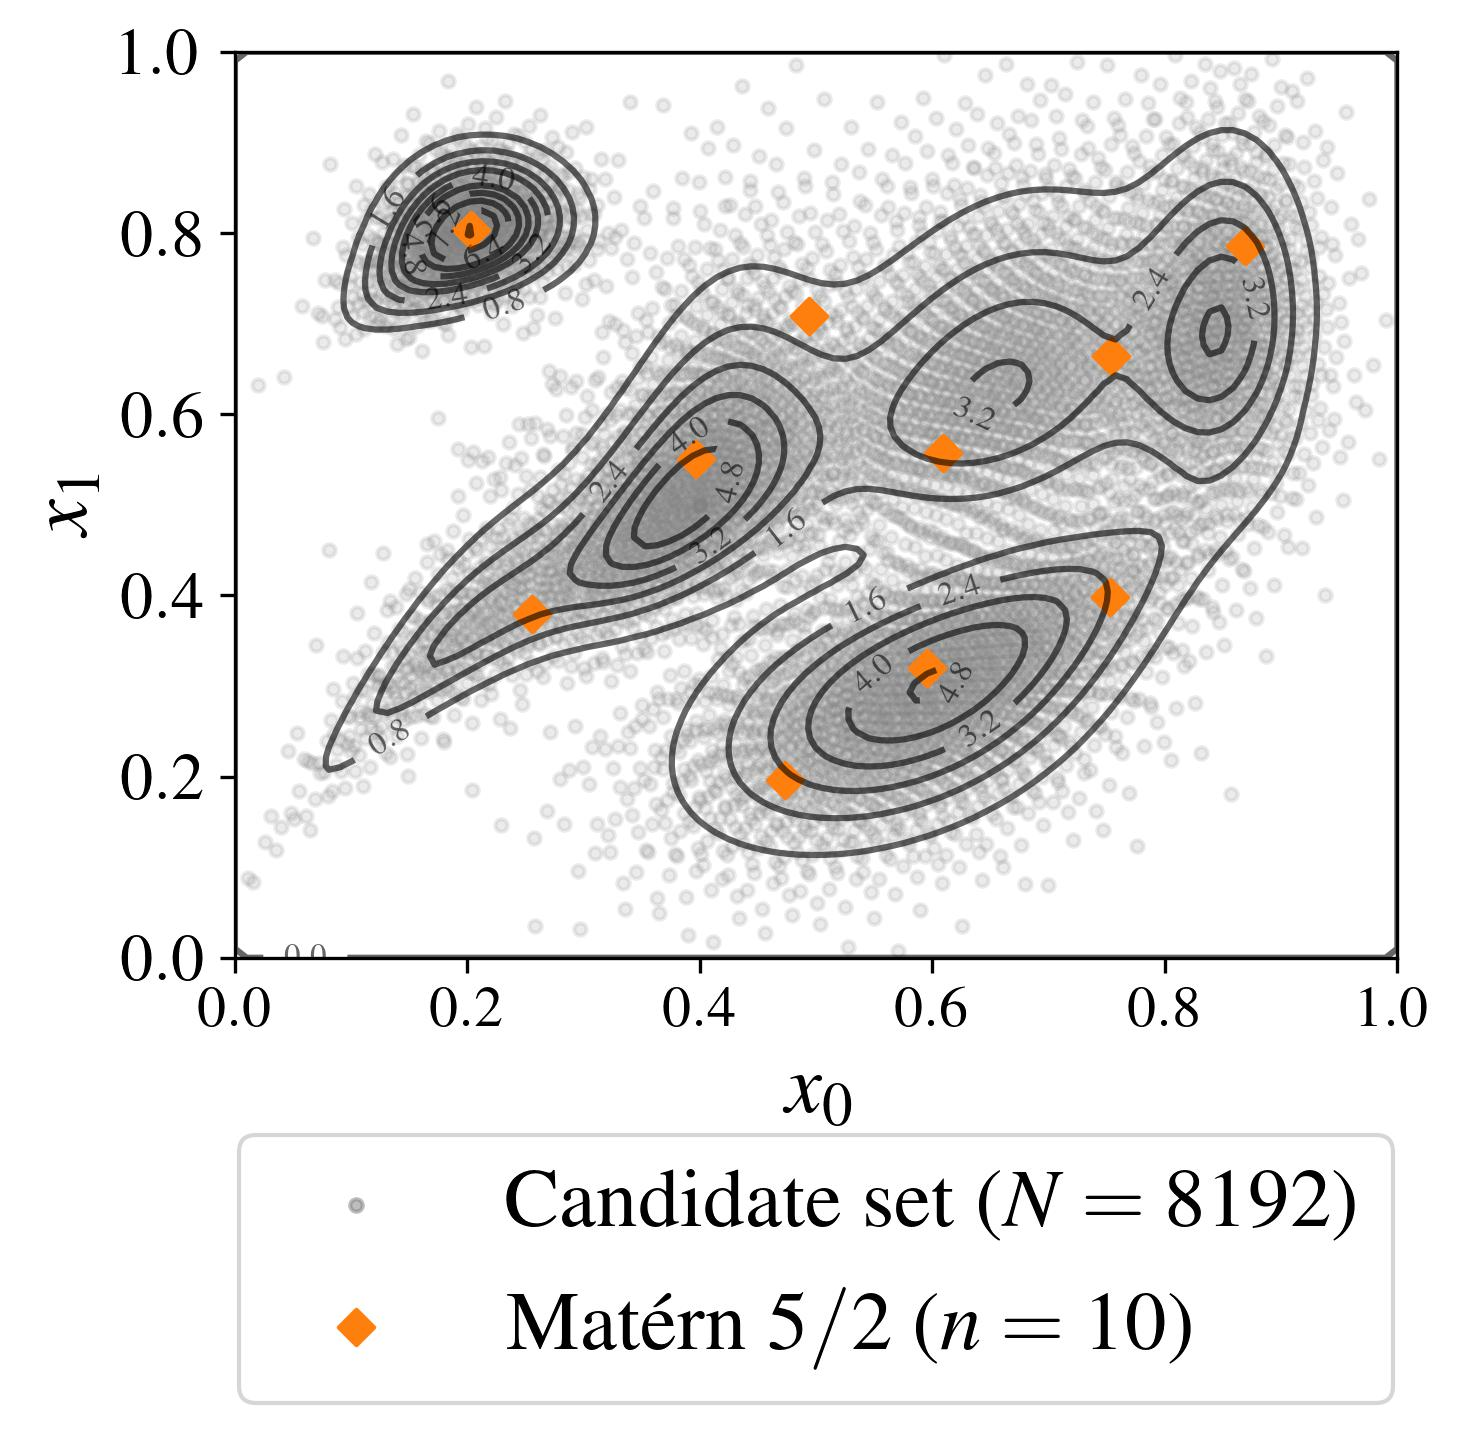
\includegraphics[width=0.32\textwidth]{part2/figures/DCE/numerical_experiments/gaussian_mixture_sampling10.jpg}
    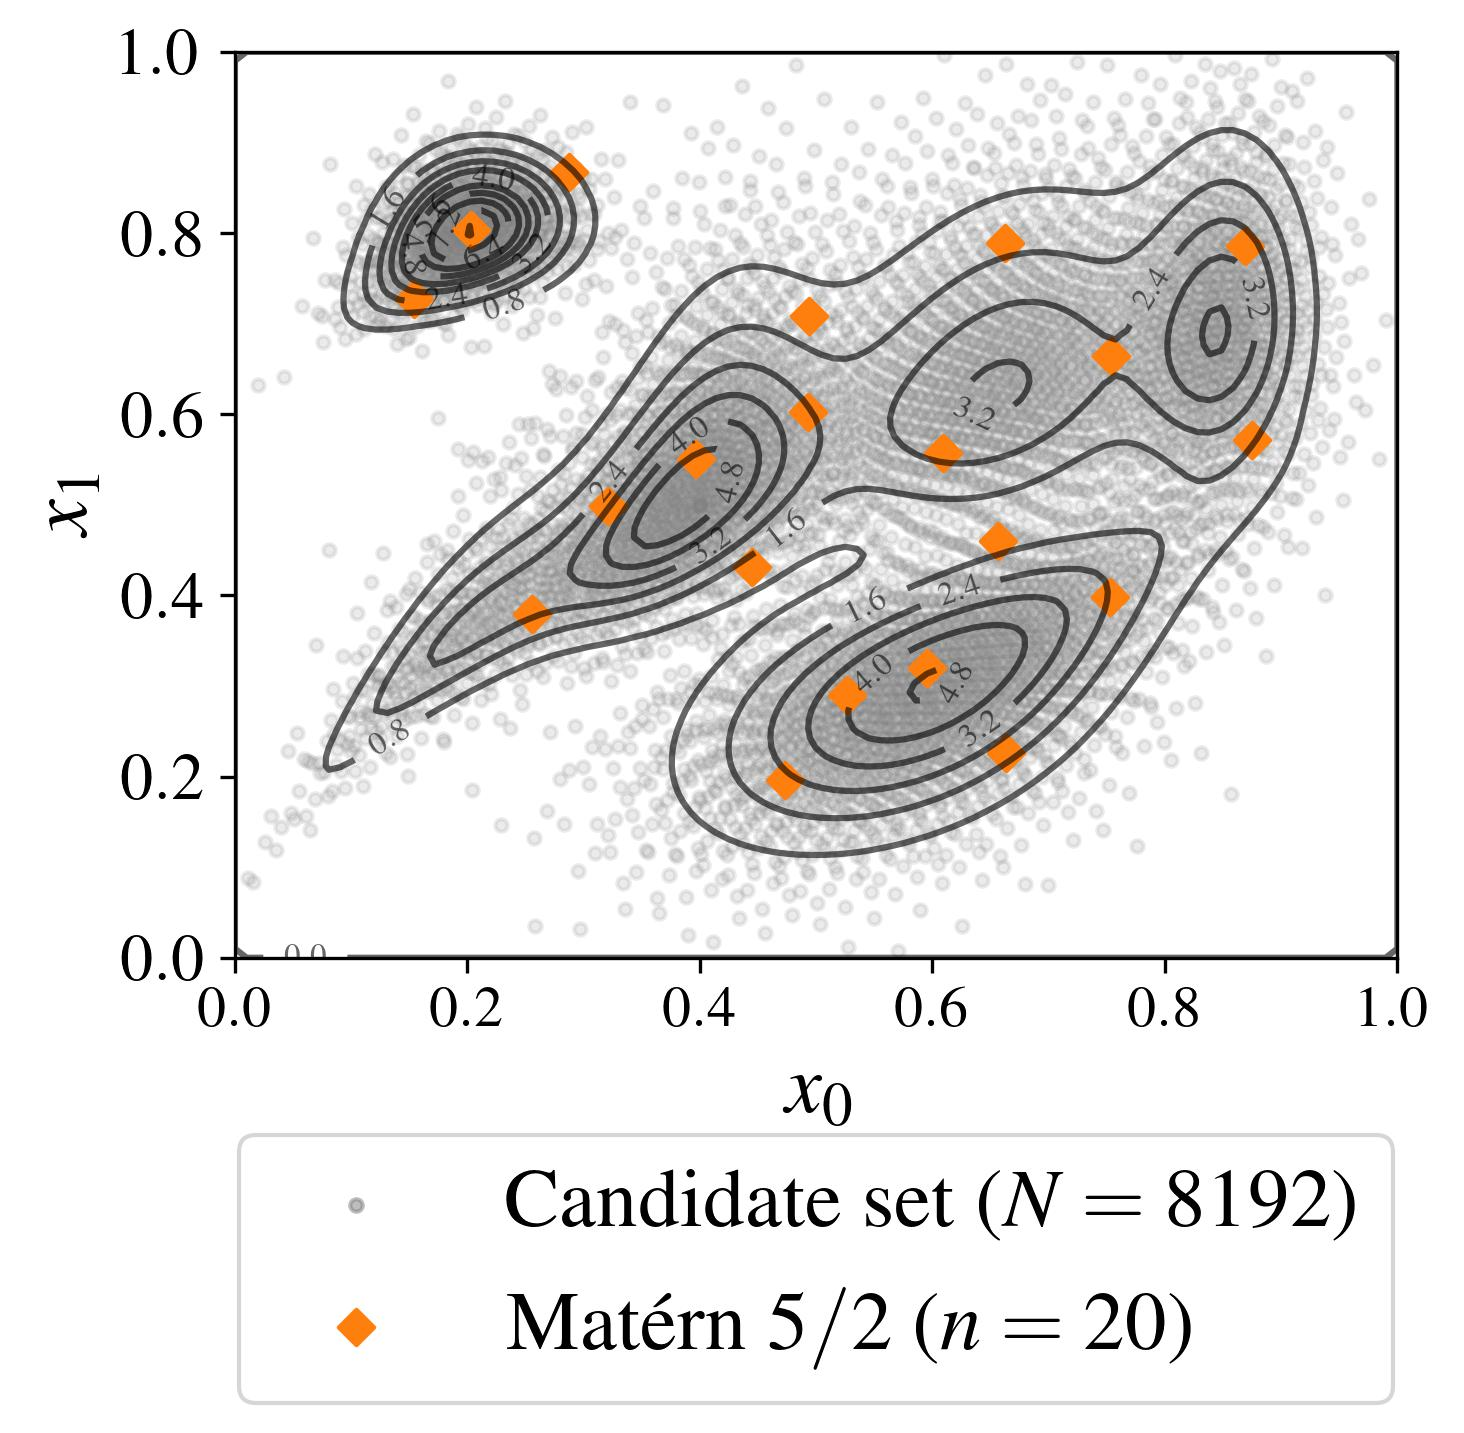
\includegraphics[width=0.32\textwidth]{part2/figures/DCE/numerical_experiments/gaussian_mixture_sampling20.jpg}
    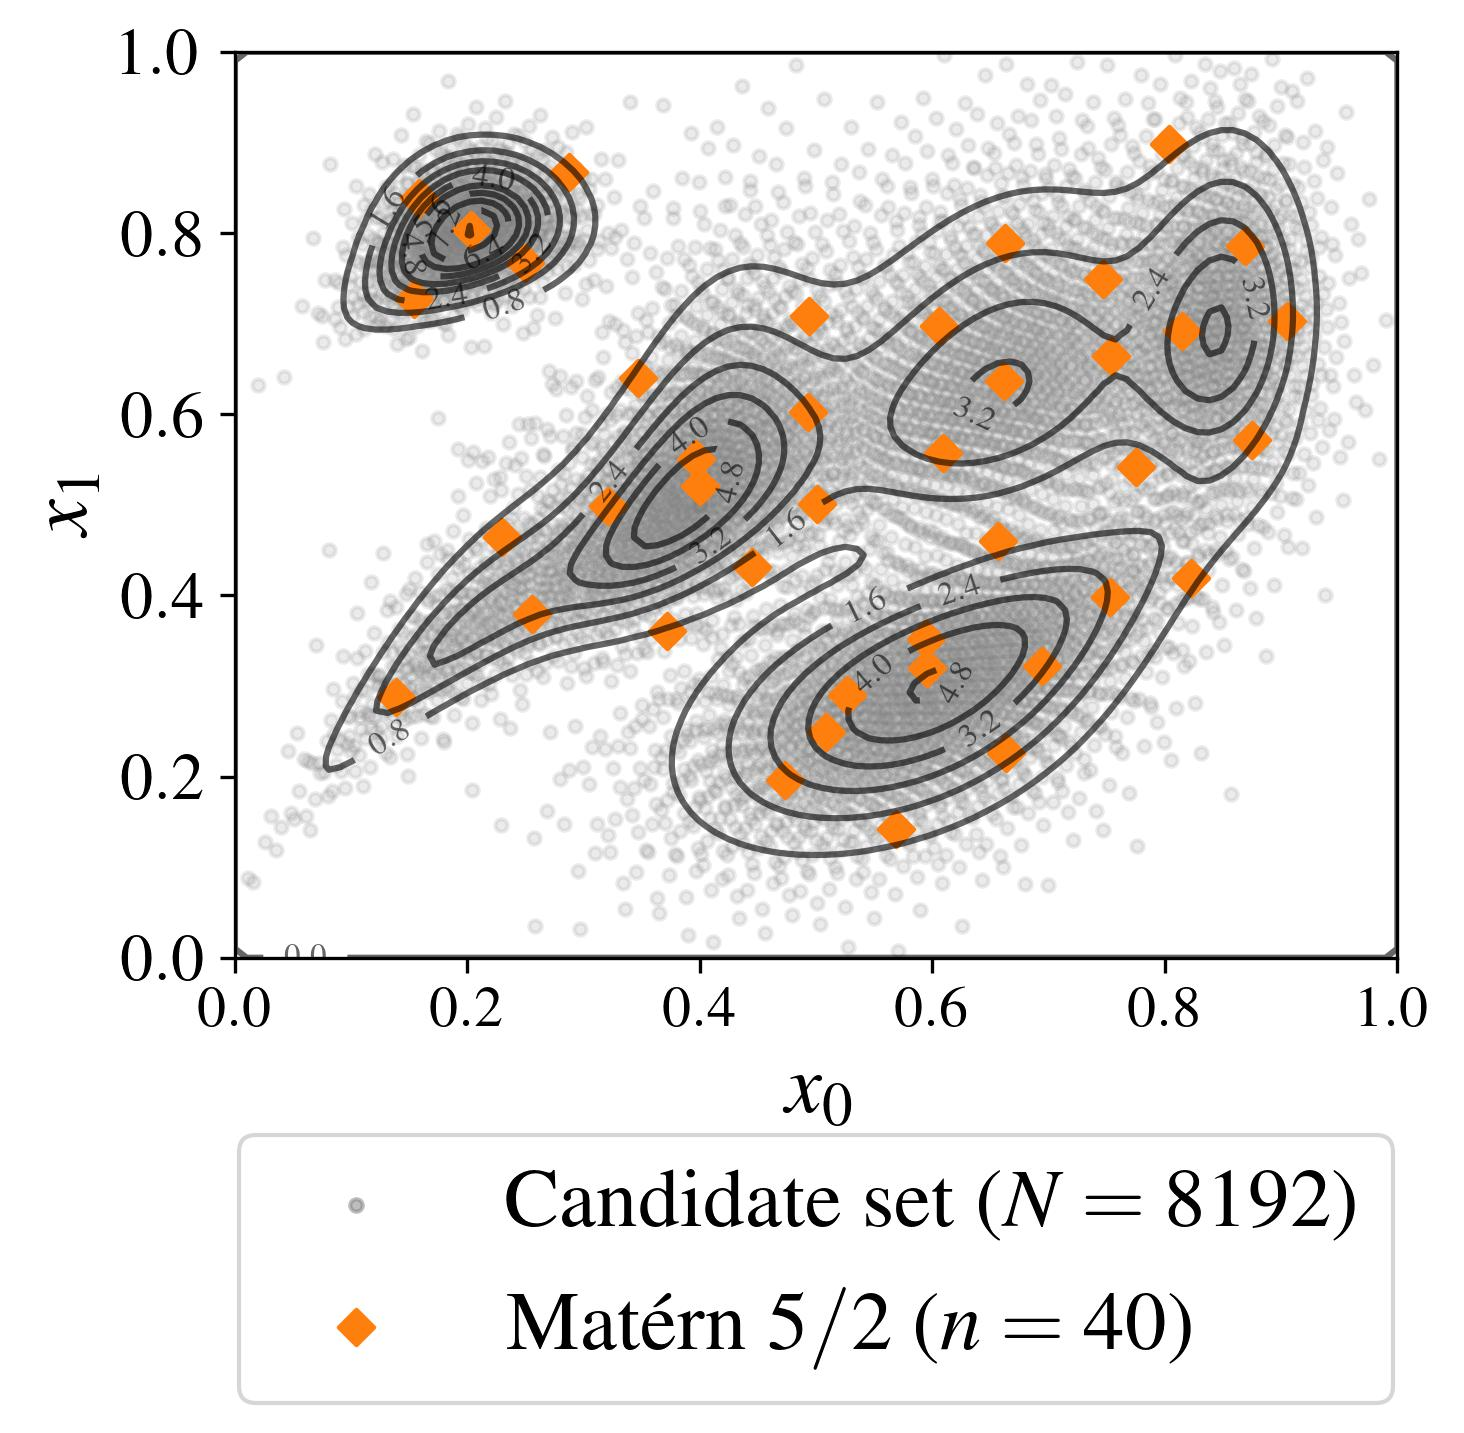
\includegraphics[width=0.32\textwidth]{part2/figures/DCE/numerical_experiments/gaussian_mixture_sampling40.jpg}
\end{center}
\caption{Sequential kernel herding for increasing design sizes ($n\in\{10, 20, 40\}$) built on a candidate set of $N=8196$ points drawn from a complex Gaussian mixture $\pi$.} \label{fig:KH_mixture}
\end{figure}

%%%%%%%%%%%%%%%%%%
Other approaches take advantage of the progressive knowledge acquired sequentially from the outputs to select the following points in the design. 
These methods are sometimes called ``active learning'' or ``adaptive strategies'' \citep{fau_2021}. 
Many of them rely on a sequentially updated Gaussian process (or Kriging) metamodel. 
To solve a probabilistic integration problem, the concept of Bayesian quadrature is introduced in the following. 

%Mention KSD and Greedy Stein points? Cite \cite{teymur_gorham_2021}?

%------------------------------------------------------------%
\subsection{Bayesian quadrature}
%------------------------------------------------------------%
\paragraph{Gaussian processes for Bayesian quadrature}%------%

Kernel methods and Gaussian processes present a lot of connections and equivalences, thoroughly reviewed by \cite{motonobu_2018}. 
In numerical integration, Gaussian processes have been used to build quadrature rules in the seminal paper of \cite{ohagan_1991}, introducing the concept of \emph{Bayesian quadrature} (\abv{bq}). 
Let us recall the probabilistic integration problem $I_\pi(g) = \int_{\iD_\bX} g(\bx) \dd \pi(\bx)$ (stated in \eq{eq:quadrature_rule}). 
From a general point of view, this quantity could be generalized by composing $g$ with another function $\psi$ (e.g., other moments, quantiles, exceedance probabilities). 
The quantity of interest then becomes, $I_\pi(\psi(g))$, for example when $\psi$ is a monomial, it gives a moment of the output distribution.

Let us assume, adopting a Bayesian point of view, that $G$ is a stochastic process describing the uncertainty affecting the knowledge about the true function $g$. 
Let $G$ be a Gaussian process (GP) prior with a zero trend (denoted by $\textbf{0}$) to ease the calculation, and a stationary covariance kernel (denoted by $k(\cdot, \cdot)$). 
The conditional posterior $G_n = (G | \by_n) \sim \GP(\eta_n, s_n^2)$ has been conditioned on the function observations $\by_n = \left[g\left(\bx^{(1)}\right), \ldots, g\left(\bx^{(n)}\right)\right]\TT$ computed from the input design $\bX_n$ and is fully defined by the well-known ``Kriging equations'' (see e.g., \citealp{rasmussen_2006}):
\begin{equation}
    \left\{
    \begin{array}{ll}
        \eta_n(\bx) &= \bk_n\TT(\bx) \bK_n^{-1} \by_n\\
        s_n^2(\bx) &= k_n(\bx, \bx) - \bk_n\TT(\bx) \bK_n^{-1} \bk_n(\bx)
    \end{array}
\right.
\label{eq:kriging}
\end{equation}
where $\bk_n(\bx)$ is the column vector of the covariance kernel evaluations $[k_n(\bx, \bx^{(1)}), \dots,\allowbreak k_n(\bx, \bx^{(n)})]$ and $\bK_n$ is the $(n \times n)$ variance-covariance matrix such that the $(i, j)$-element is $\left\{\bK_n \right\}_{i, j}=k_n(\bx^{(i)}, \bx^{(j)})$.

In BQ, the main object is the random variable $I_{\pi}(G_n)$. 
According to \cite{briol_oates_2019}, its distribution on $\R$ is the pushforward of $G_n$ through the integration operator $I_\pi(\cdot)$, sometimes called \emph{posterior distribution}: 
\begin{equation}
    I_{\pi}(G_n) = \int_{\iD_\bX} (G(\bx) | \by_n)  \dd \pi(\bx) = \int_{\iD_\bX} G_n(\bx)  \dd \pi(\bx) \,.
\label{eq:posterior}
\end{equation}

\fig{fig:bayesian_quad} provides a one-dimensional illustration of the Bayesian quadrature of an unknown function (dashed black curve) against a given input measure $\pi$ (with corresponding grey distribution at the bottom). 
For an arbitrary design, one can fit a Gaussian process model, interpolating the function observations (black crosses). 
Then, multiple trajectories of this conditioned Gaussian process $G_n$ are drawn (orange curves) whilst its mean function, also called ``predictor'', is represented by the red curve. 
Therefore, the input measure $\pi$ is propagated through the conditioned Gaussian process to obtain the random variable $I_{\pi}(G_n)$, with distribution represented on the right plot (brown curve). 
Again on the right plot, remark how the mean of this posterior distribution (brown line) is closer to the reference output expected value (dashed black line) than the arithmetic mean of the observations (black line). 
This plot was inspired by the paper of \cite{husar_duvenaud_2012}.

\begin{figure}[!h]
\begin{center}
    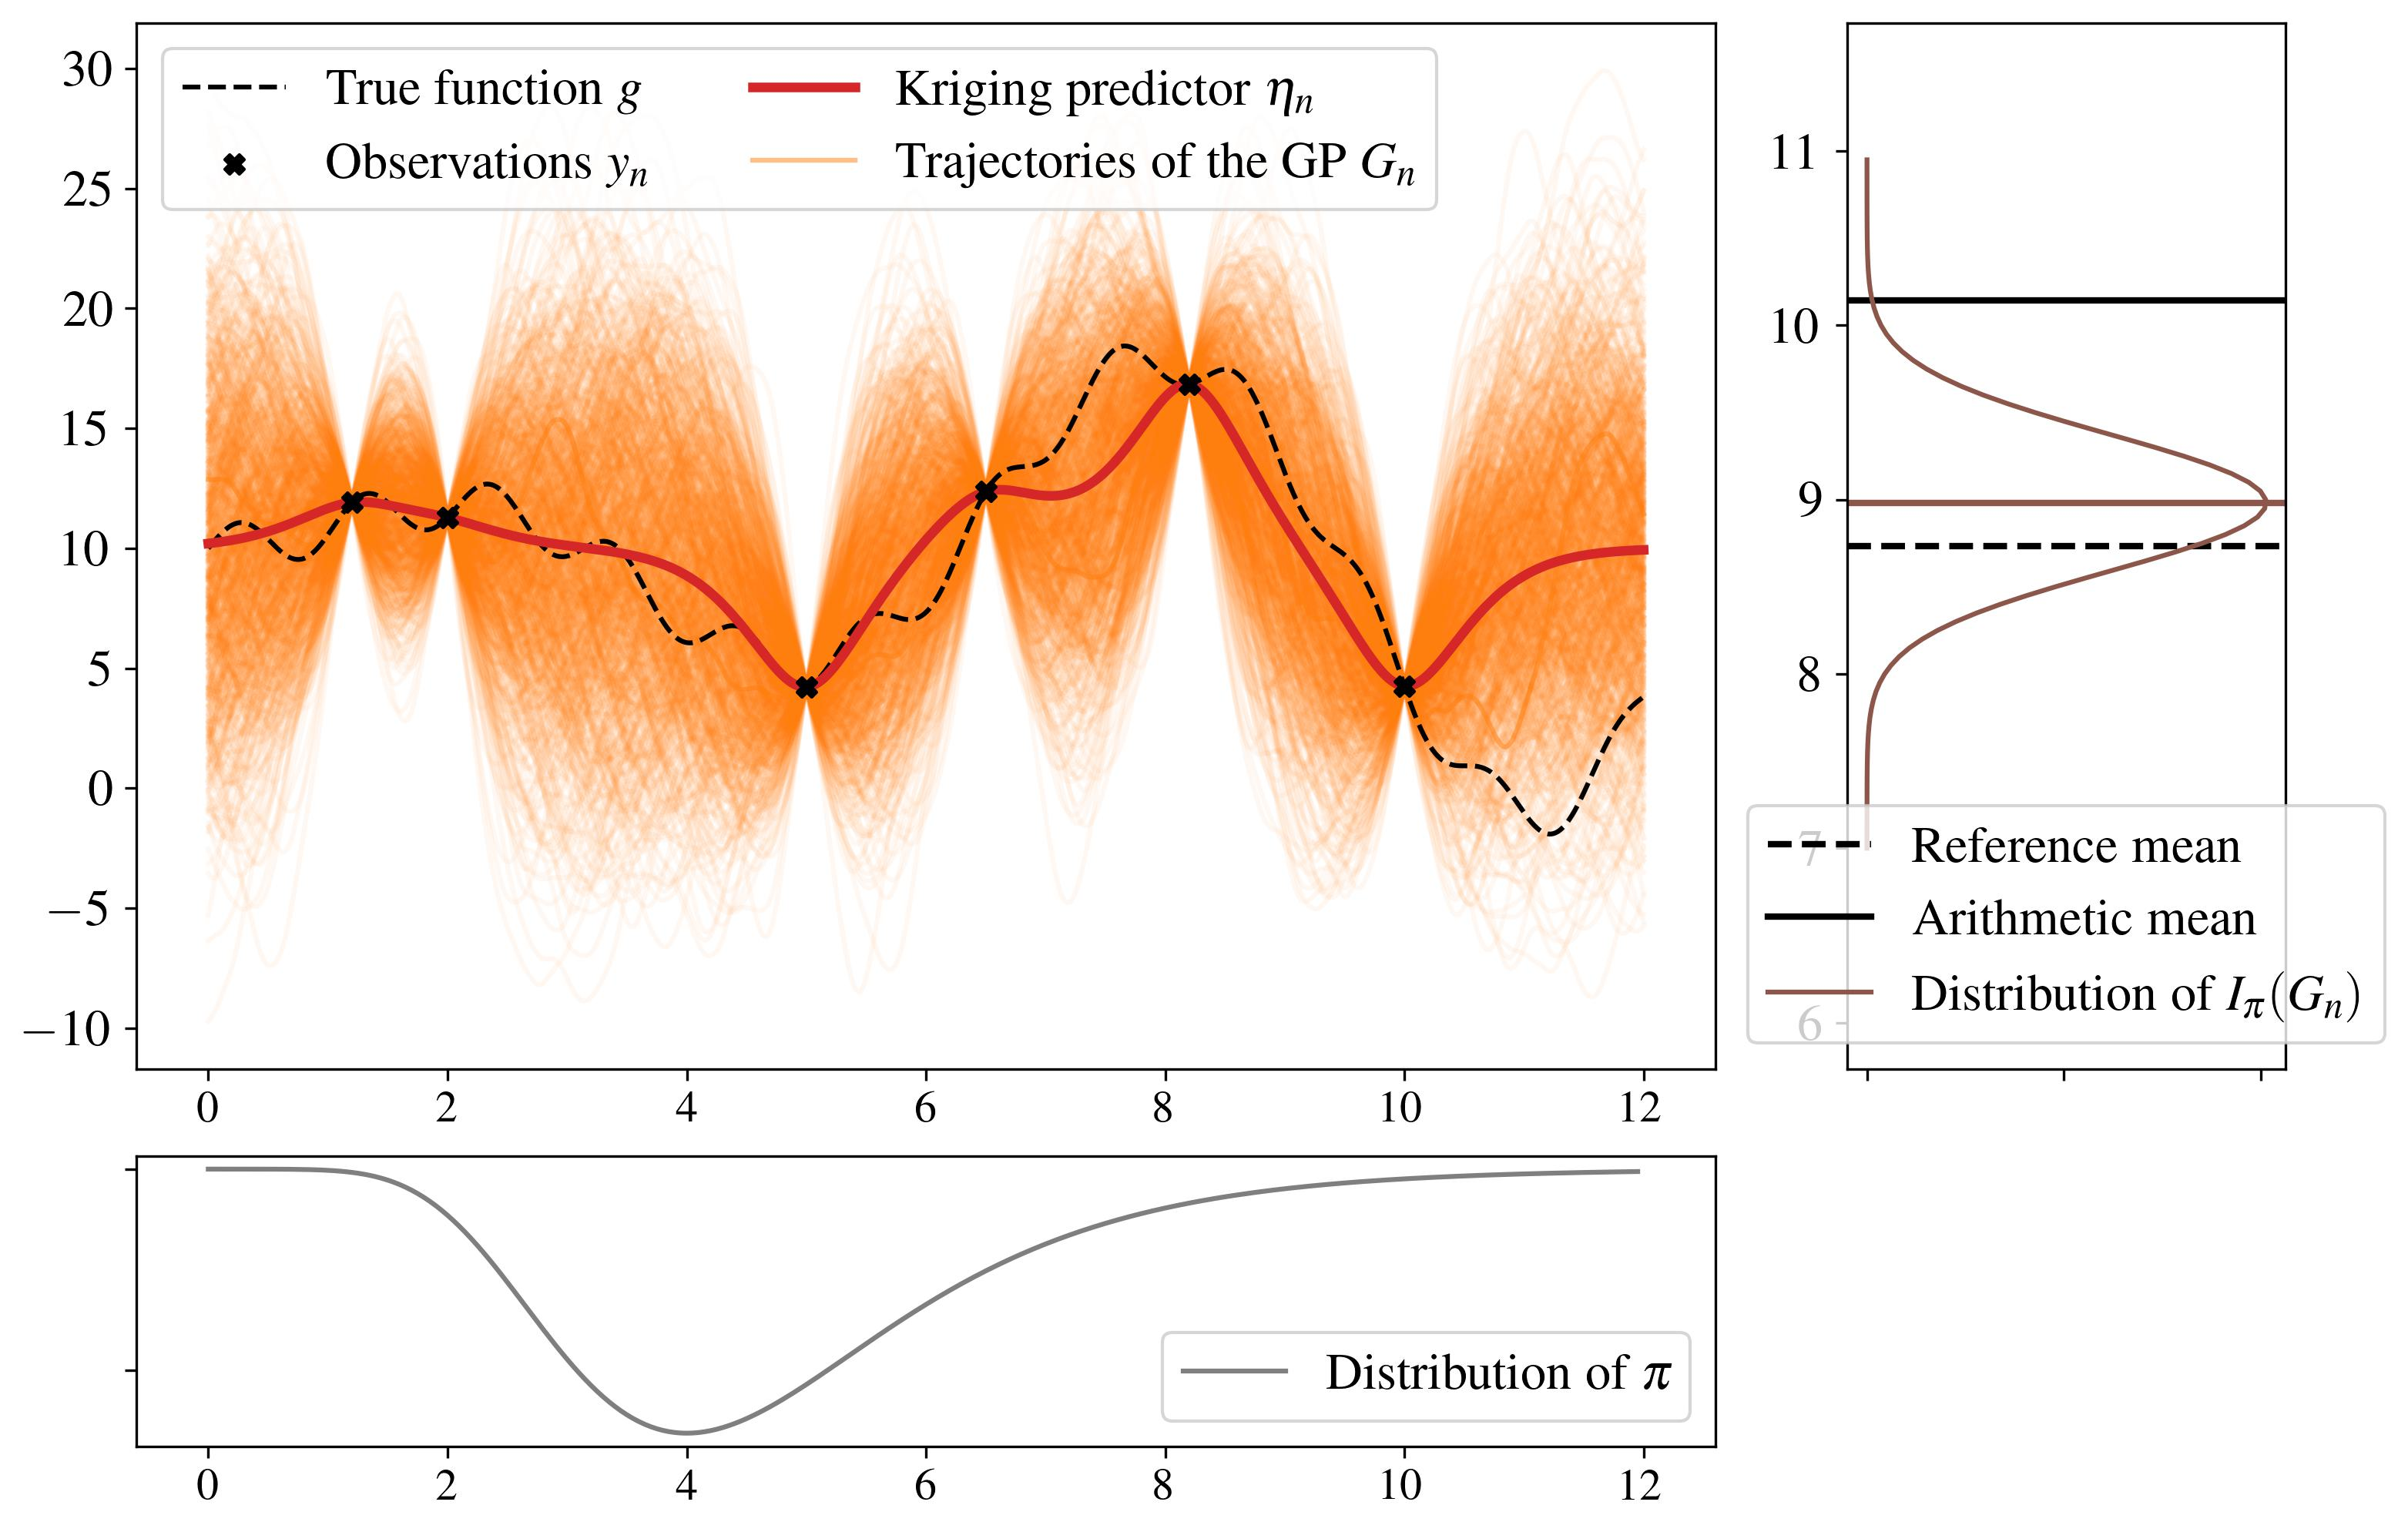
\includegraphics[width=0.7\textwidth]{part2/figures/DCE/numerical_experiments/posterior_distribution_centered.jpg}
    \caption{Bayesian quadrature on a one-dimensional case.}
    \label{fig:bayesian_quad}
\end{center}
\end{figure}

\paragraph{Optimal weights computed by Bayesian quadrature}%---------------------%
Taking the random process $G_n$ as Gaussian conveniently implies that its posterior distribution $a_\pi(G_n)$ is also Gaussian. 
This comes from the linearity of the infinite sum of realizations of a Gaussian process. 
The posterior distribution is described in a closed form through its mean and variance by applying Fubini's theorem (see the supplementary materials from \citealp{briol_oates_2019} for the proof regarding the variance): 
\begin{equation}
     \overline{y}_n^{\mathrm{BQ}} = \E\left[I_{\pi}(G_n) | \by_n \right] 
     = \int_{\iD_\bX} \eta_n(\bx) \dd \pi(\bx)
     = \left[\int_{\iD_\bX} \bk_n\TT(\bx) \dd \pi(\bx) \right] \bK_n^{-1} \by_n
     = P_\pi(\bX_n) \bK_n^{-1} \by_n,       
\label{eq:mean_post}
\end{equation}

\begin{equation}
    \left(\sigma_n^{\mathrm{BQ}}\right)^2 = \var\left(I_{\pi}(G_n) \right) 
    = \iint_{\iD_{\bX^2}} k_n(\bx, \bx') \dd \pi(\bx) \dd \pi(\bx') 
    = \varepsilon_\pi - P_\pi(\bX_n) \bK_n^{-1} P_\pi(\bX_n)\TT.
\label{eq:var_post}
\end{equation}
\noindent
Where $P_\pi(\bX_n)$ is the row vector of potentials $\left[\int k_n(\bx, \bx^{(1)}) \dd \pi(\bx), \dots, \int k_n(\bx, \bx^{(n)}) \dd \pi(\bx)\right]$, and $\varepsilon_\pi$ is given in \eq{eq:target_energy}. 
As in the one-dimensional example presented in \fig{fig:bayesian_quad}, the expected value of $I_{\pi}(G_n)$ expressed in \eq{eq:mean_post} is a direct estimator of the quantity of interest \eq{eq:quadrature_rule}. 
The so-called ``Bayesian quadrature estimator'' appears to be a simple linear combination of the observations by taking the row vector of ``optimal weights'' as: 
\begin{equation}
    \wBQ = P_\pi(\bX_n) \bK_n^{-1}
    \label{eq:bq_weights}
\end{equation}
For any given sample, an optimal set of weights can be computed, leading to the mean of the posterior distribution. 
Remark here that this enhancement depends on the evaluation of the inverse variance-covariance matrix $\bK_n^{-1}$, which can present numerical difficulties, either when design points are too close, making the conditioning bad. 
Moreover, a prediction interval on the BQ estimator can be computed since the posterior distribution is Gaussian, with a variance expressed in closed-form in \eq{eq:var_post}. 
The expressions in \eq{eq:mean_post} and \eq{eq:var_post} were extended to Gaussian processes in the case of constant and linear trends in \cite{pronzato_zhigljavsky_2020}. 
In the following numerical experiments, the expression with a hypothesis of constant trend $\beta_n$ is used, which leads to:
\begin{equation}
     \E\left[I_{\pi}(G_n)\right] = \beta_n + P_\pi(\bX_n) \bK_n^{-1} \left(\by_n - \beta_n \mathbf{1}_n \right).
     \label{eq:mean_post_cst}
\end{equation}

\noindent Then, an a posteriori 95\% prediction interval around the mean Bayesian estimator is directly given by: 
\begin{equation}
   \overline{y}_n^{\mathrm{BQ}} \in \left[\overline{y}_n^{\mathrm{BQ}} - 2\sigma_n^{\mathrm{BQ}}, \overline{y}_n^{\mathrm{BQ}} + 2\sigma_n^{\mathrm{BQ}} \right].
\end{equation}

\paragraph{Variance-based Bayesian quadrature rule}%----------------%
The link between the posterior variance and the squared MMD has been first made by \cite{husar_duvenaud_2012} in their Proposition 1: the expected variance in the Bayesian quadrature $\var\left(I_{\pi}(G_n)\right)$ is the MMD between the target distribution $\pi$ and $\zeta_n = \sum_{i=1}^n \wBQ^{(i)} \delta(\bx^{(i)})$. 
The proof is reproduced below (as well as in Proposition 6.1 from \citealp{motonobu_2018}): 
\begin{subequations}
\begin{align}
    \var\left(I_{\pi}(G_n)\right) &= \E\left[ \left(I_{\pi}(G_n) - I_{\zeta_n}(G_n)\right)^2\right]\\
    &= \E\left[ \left( \left\langle G_n, P_{\pi} \right\rangle_{\iH(k)} - \left\langle G_n, P_{\zeta_n}\right\rangle_{\iH(k)} \right)^2\right]\\ \label{eq:bq_v1}
    &= \E\left[ \left\langle G_n, P_{\pi} - P_{\zeta_n} \right\rangle_{\iH(k)}^2\right]\\ \label{eq:bq_v2}
    %&= \E\left[ \lVert G_n \lVert^2 + \lVert P_{\pi}(\bx) - P_{\zeta_n}(\bx) \lVert^2 - 2 \left\langle G_n, P_{\pi}(\bx) - P_{\zeta_n}(\bx) \right\rangle_{\iH(k)}\right]\\
    &= \lVert P_{\pi} - P_{\zeta_n} \lVert^2_{\iH(k)}\\ 
    &= \MMD(\pi, \zeta_n)^2.
\end{align}
\end{subequations}
Note that the transition from equation \eq{eq:bq_v1} to \eq{eq:bq_v2} relies on the property stating that if $G$ is a standard Gaussian process then $\forall g \in \iH(k) : \left\langle G, g \right\rangle_{\iH(k)} \sim \iN(0, \lVert g \lVert^2_{\iH(k)}$). 
The method that sequentially builds a quadrature rule by minimizing this variance is called by the authors ``sequential Bayesian quadrature''. 
According to the previous proof, this criterion can be seen as an optimally-weighted version of the kernel herding criterion, as stated in the title of the paper from \cite{husar_duvenaud_2012}. 
Later, \cite{briol_2015} proved the weak convergence of $I_{\pi}(G_n)$ towards the target integral. 
Closer to wind turbine applications, \cite{huchet_2019} and \cite{huchet_mattrand_2019} introduced the ``Adaptive Kriging Damage Assessment'' method: a Kriging-based method for mean damage estimation that is very close to sequential Bayesian quadrature. 
However, This type of method inherits the limits from both KH and BQ since it searches for optimal design points among a candidate set and computes an inverse variance-covariance matrix. 
These numerical operations both scale hardly in high dimension. 

\medskip
\begin{remark}
Every quadrature method introduced in this section has been built without any observation of the possibly costly function $g$. 
Therefore, they cannot be categorized as active learning approaches. 
Contrarily, \cite{motonobu_2019} presents a set of methods for BQ with transformations (i.e., adding a positivity constraint on the function $g$), which are truly active learning methods. 
\end{remark}

%In the end, active methods are not widely used for numerical integration \citep{wei_2020,goncalves_batchvarov_2020}, and from a general point of view, one can wonder in which situation the active learning framework presents a actual added value. 

%Apart from some very specific problems (e.g., contour finding of a limit-state function in reliability analysis \citep{echard_2011}. 

%\begin{remark}
%As much as the previous criteria will reduce the posterior variance, the estimation error may present a bias.
%\end{remark}

%============================================================%
%============================================================%
\section{Numerical experiments}\label{sec:sec44}
%============================================================%
%============================================================%
This section presents numerical results computed on two different analytical toy cases, respectively in dimension 2 (toy case \#1) and dimension 10 (toy case \#2), with easy-to-evaluate functions $g(\cdot)$ and associated input distributions $\pi$. 
Therefore, reference values can easily be computed with great precision. 
For each toy case, a large reference Monte Carlo sample ($N_{\mathrm{ref}} = 10^8$) is taken. 
This first benchmark compares the mean estimation of toy cases given by a quasi-Monte Carlo technique (abbreviated by QMC in the next figures) which consists herein using a Sobol' sequence, and kernel herding with the three kernels defined in Table \ref{tab:kernels}. 
Notice that the quasi-Monte Carlo designs are first generated on the unit hypercube and then, transformed using the generalized Nataf transformation to follow the target distribution \citep{lebrun_2009}. 
Additionally, the performances of kernel herding for both uniform and optimally-weighted \eq{eq:mean_post_cst} estimators are compared.


All the following results and methods (i.e., the kernel-based sampling and BQ methods) have been implemented in a new open source Python package named \texttt{otkerneldesign\footnote{\href{https://efekhari27.github.io/otkerneldesign/master/index.html}{https://efekhari27.github.io/otkerneldesign/master/index.html}}}. 
This development mostly relies on the open source software \ots(``Open source initiative for the Treatment of Uncertainties, Risks'N Statistics'') devoted to uncertainty quantification and statistical learning \citep{baudin_dutfoy_2017}. 
Finally, note that the numerical experiments for the toy cases are available in the Git repository named \texttt{ctbenchmark}\footnote{\href{https://github.com/efekhari27/ctbenchmark}{https://github.com/efekhari27/ctbenchmark}}. 


%------------------------------------------------------------%
\subsection{Benchmark results on analytical test cases}
%------------------------------------------------------------%
The toy cases were chosen to cover a large panel of complex probabilistic integration problems, completing the ones from \cite{fekhari_renew_2022}.
To assess the complexity of numerical integration problems, \cite{owen_2003} introduced the concept of the ``effective dimension'' of an integrand function (number of the variables that actually impact the integral). 
The author showed that functions built on sums yield a low effective dimension (unlike functions built on products). 
In the same vein, \cite{kucherenko_feil_2011} build three classes of integrand sorted by difficulty depending on their effective dimension: \begin{itemize}
    \item \emph{class A}: problem with a few dominant variables.
    \item \emph{class B}: problem without unimportant variables, and important low-order interaction terms.
    \item \emph{class C}: problems without unimportant variables, and important high-order interaction terms. 
\end{itemize}
The 10-dimensional ``GSobol function'' (toy case \#2) with a set of coefficient $\{a_i=2\}_{i=1}^{10}$ has an effective dimension equal to 10 and belongs to the hardest class C from \cite{kucherenko_feil_2011}. 
In the case of the two-dimensional Gaussian mixture problem, the complexity is carried by the mixture of Gaussian distributions with highly nonlinear dependencies.
Probabilistic integration results are presented in \fig{fig:test case1} (toy case \#1) and \fig{fig:test case2} (toy case \#2). 
Kernel herding samples using the energy-distance kernel are in red, while quasi-Monte Carlo samples built from Sobol' sequences are in grey. 
Convergences of the arithmetic means are plotted on the left and MMDs on the right. 
The respective BQ estimators of the means are plotted in dashed lines. 

\begin{table*}
    \centering
    \caption{Analytical test cases}
    \begin{tabular}{llll}
     \hline
        \textbf{Test case \#1} & $dim = 2$ & $g_1(\bx)= x_1 + x_2$ & Gaussian mixture from \fig{fig:KH_mixture} \\
        \textbf{Test case \#2} & $dim = 10$ & $g_2(\bx) = \prod_{i=1}^{10} \frac{|4 x_i - 2| + a_i}{1 + a_i}, \{a_i=2\}_{i=1}^{10}$ & Gaussian $\iN(\mathbf{0.5},\mathbf{I}_{10})$\\
    \end{tabular}
    \label{tab:toycases}
\end{table*}

\medskip
\begin{remark}
    Different kernels are used in these numerical experiments. 
    First, the generation kernel is used by the kernel herding algorithm to generate designs (with the heuristic tuning defined in Section~\ref{sec:4khsubsec}). 
    Second, the BQ kernel allows computation of the optimal weights (arbitrarily set up as a Matérn $5/2$ with the heuristic tuning). 
    Third, the evaluation kernel must be common to allow a fair comparison of the computed MMD results (same as the BQ kernel).
\end{remark}
\medskip

\noindent\emph{Results analysis for toy case \#1.} Convergence plots are provided in \fig{fig:test case1}. 
KH consistently converges faster than quasi-Monte Carlo in this case, especially for small sizes in terms of MMD. 
BQ weights tend to reduce the fluctuations in the mean convergence, which ensures better performance for any size. 
Overall, applying the weights enhances the convergence rate.

\smallskip
\noindent\emph{Results analysis for toy case \#2.} Convergence plots are provided in \fig{fig:test case2}. 
Although quasi-Monte Carlo is known to suffer the ``curse of dimensionality'', KH does not outperform it drastically in this example. 
In fact, KH with uniform weights performs worse than quasi-Monte Carlo while optimally-weighted KH does slightly better. 
Moreover, the results confirm that $\MMD_{\mathrm{BQ}}< \MMD_{\mathrm{unif}}$ for all our experiments. 
The application of optimal weights to the quasi-Monte Carlo sample slightly improves the estimation in this case. Note that the prediction interval around the BQ estimator is not plotted for the sake of readability. 
\smallskip

In these two toy cases, the MMD is shown to quantify numerical integration convergence well, which illustrates the validity of the inequality given in \eq{eq:quad_error}, similar to the Koksma-Hlawka inequality (as recalled in \eq{eq:KH_inequality}).

\begin{figure}[!h]
\begin{center}
    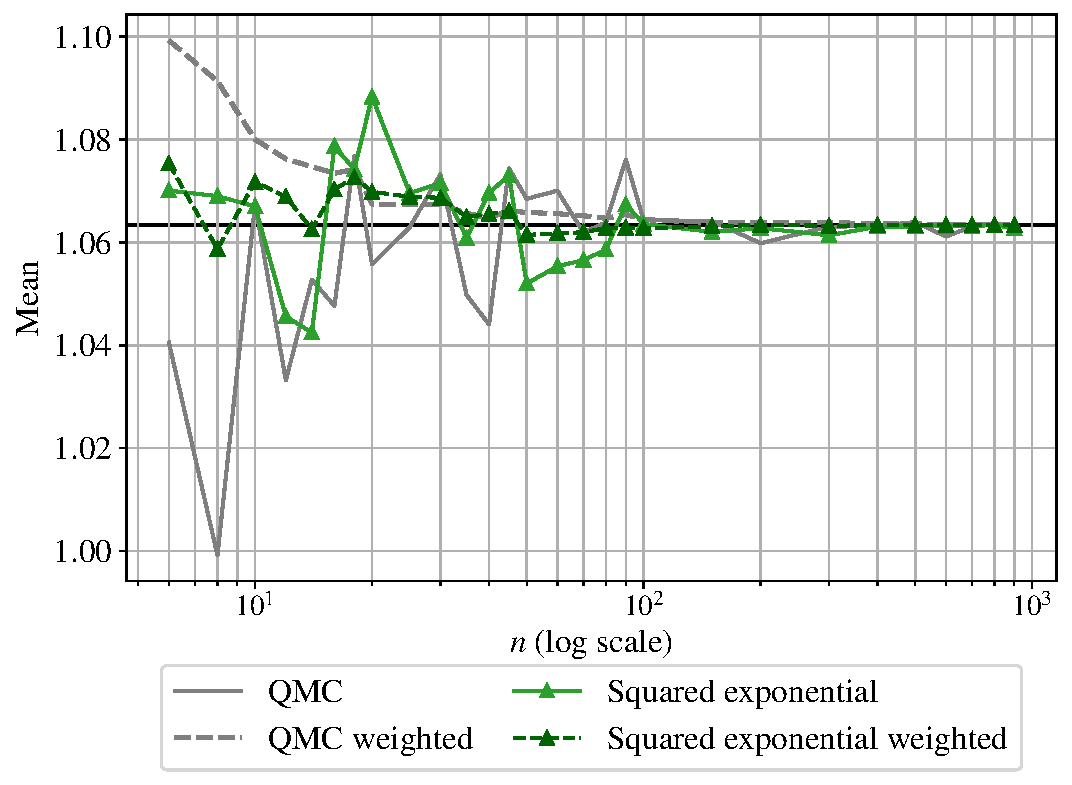
\includegraphics[width=0.48\textwidth]{part2/figures/DCE/analytical_bench/Gaussian_Mixture_convergence_SE.pdf}
    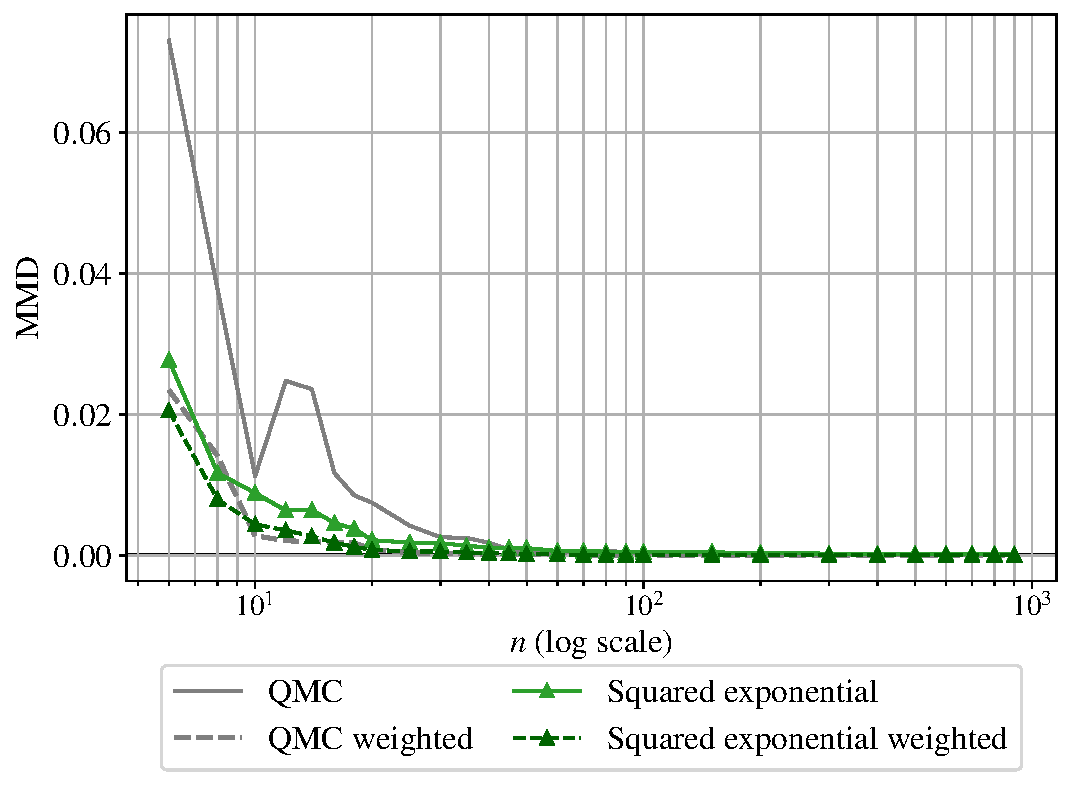
\includegraphics[width=0.48\textwidth]{part2/figures/DCE/analytical_bench/Gaussian_Mixture_convergence_MMD_SE.pdf}\\
    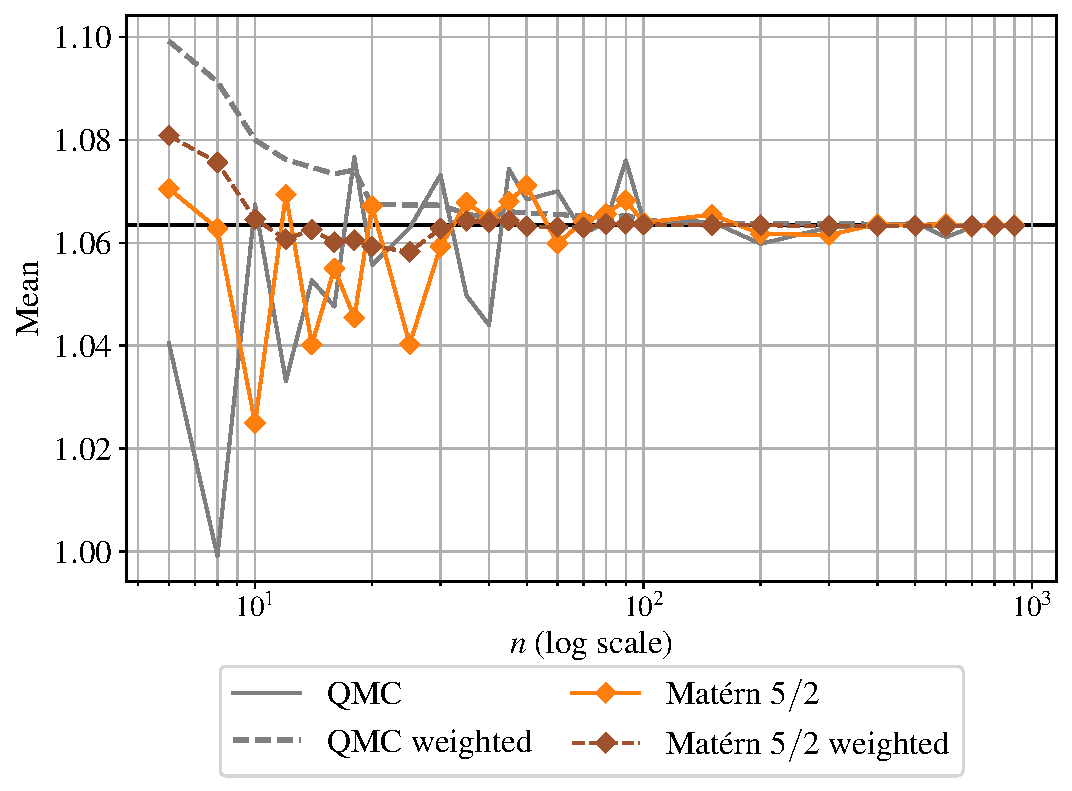
\includegraphics[width=0.48\textwidth]{part2/figures/DCE/analytical_bench/Gaussian_Mixture_convergence_Matern.pdf}
    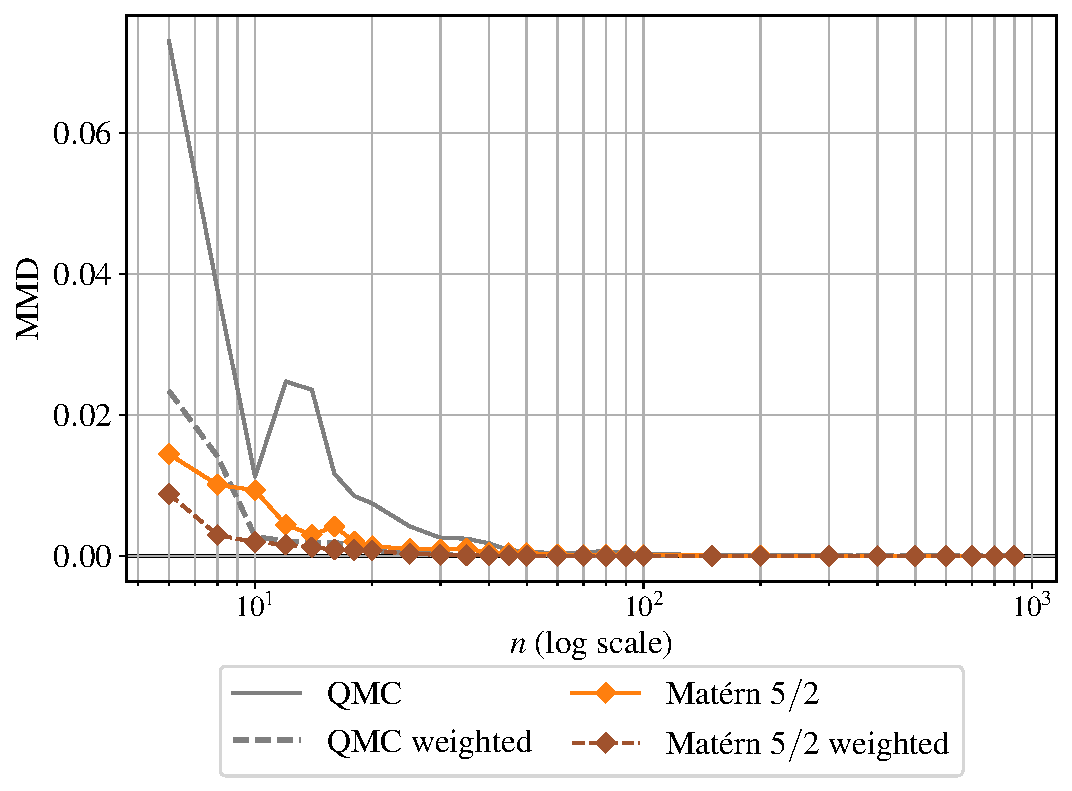
\includegraphics[width=0.48\textwidth]{part2/figures/DCE/analytical_bench/Gaussian_Mixture_convergence_MMD_Matern.pdf}\\
    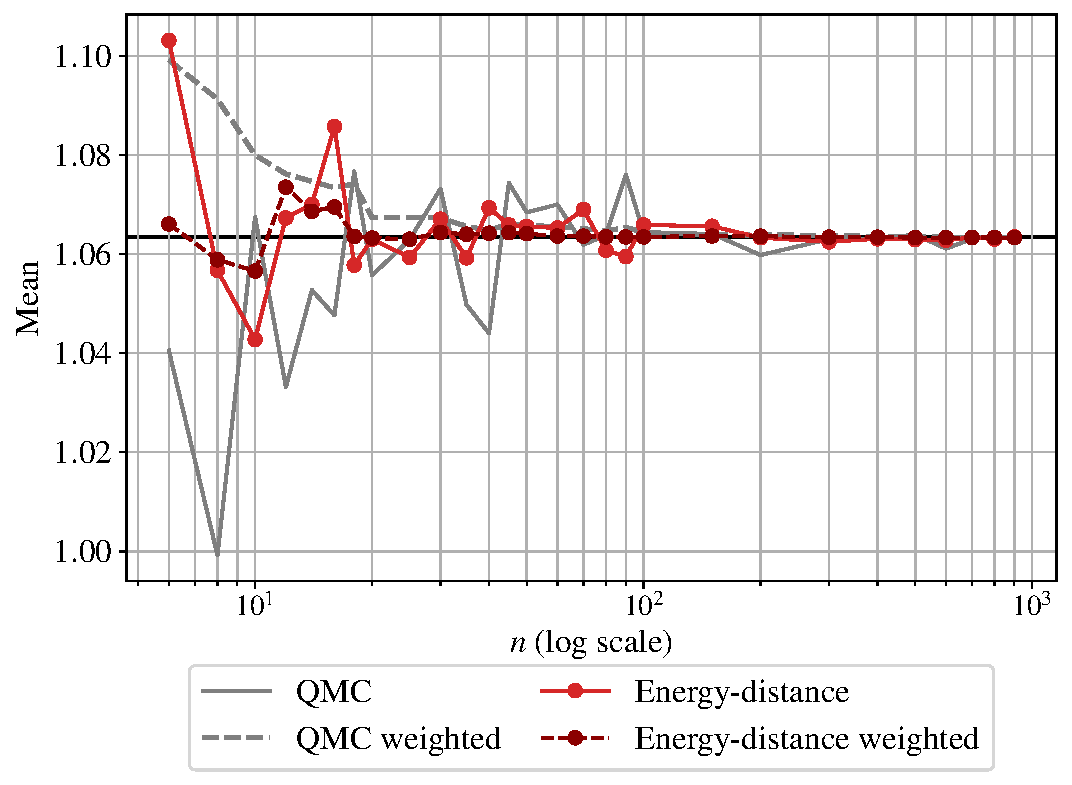
\includegraphics[width=0.48\textwidth]{part2/figures/DCE/analytical_bench/Gaussian_Mixture_convergence_ED.pdf}
    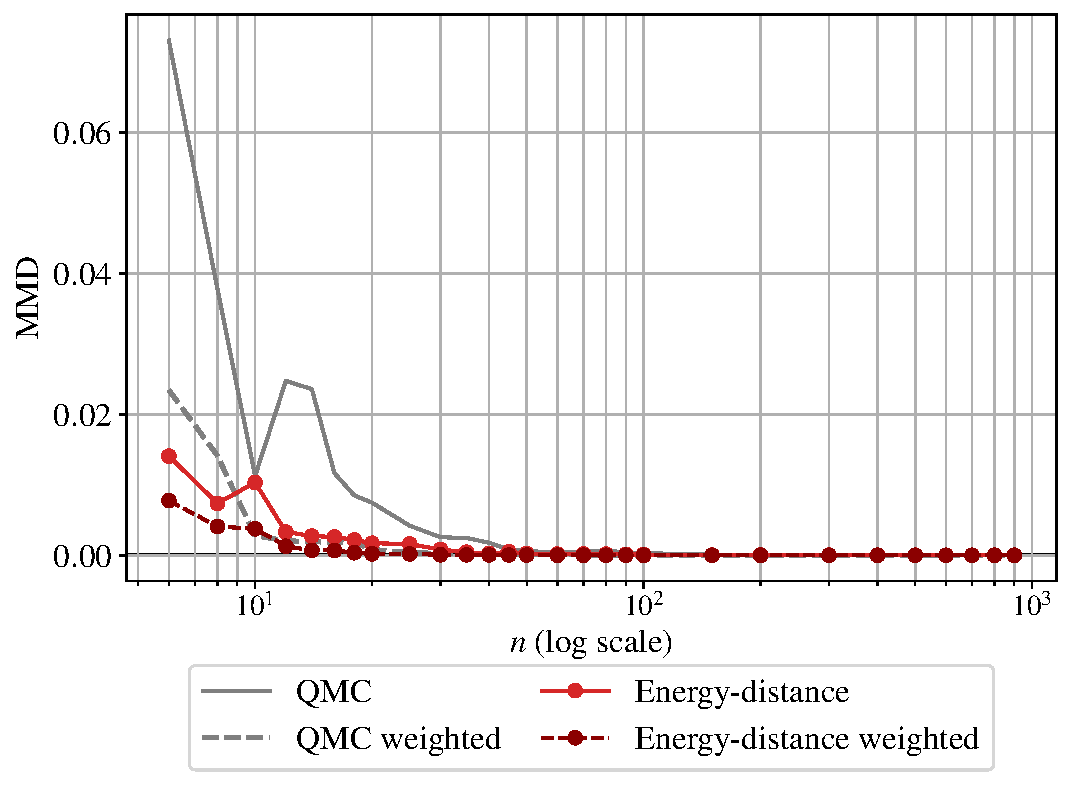
\includegraphics[width=0.48\textwidth]{part2/figures/DCE/analytical_bench/Gaussian_Mixture_convergence_MMD_ED.pdf}\\
\end{center}
\caption{Analytical benchmark results on the test case \#1.} \label{fig:test case1}
\end{figure}

\begin{figure}[!h]
\begin{center}
    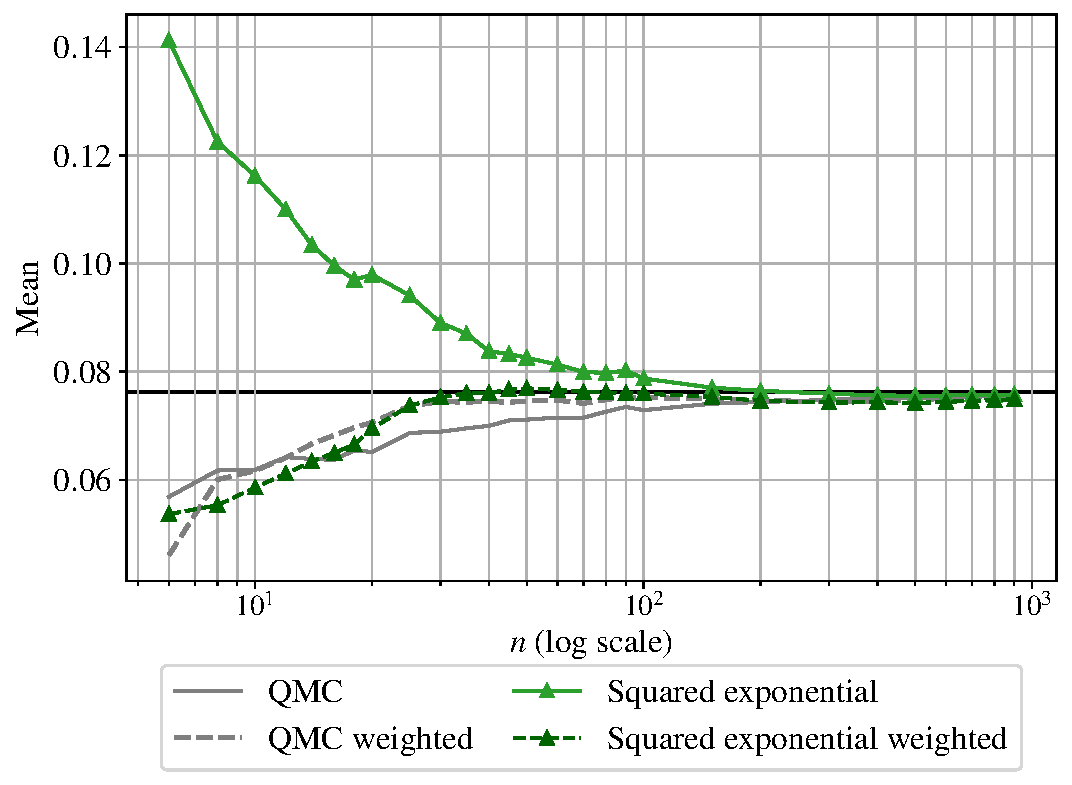
\includegraphics[width=0.48\textwidth]{part2/figures/DCE/analytical_bench/GSobol_10D_(normal_input)_convergence_SE.pdf}
    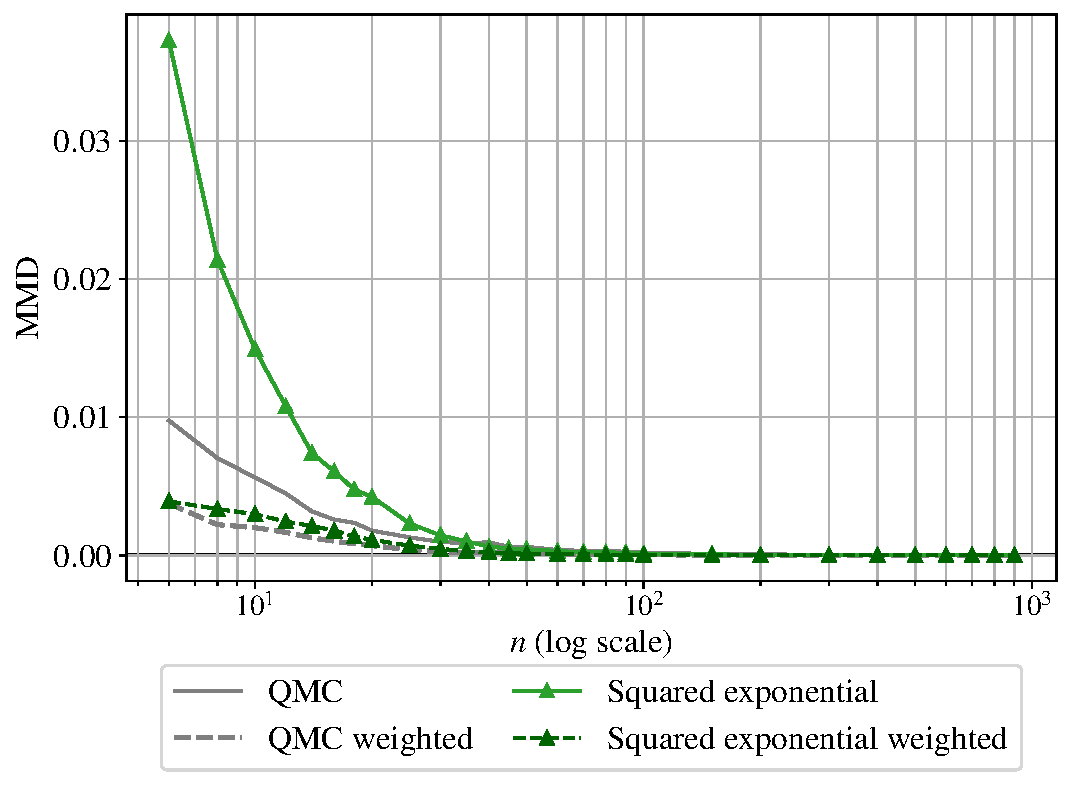
\includegraphics[width=0.48\textwidth]{part2/figures/DCE/analytical_bench/GSobol_10D_(normal_input)_convergence_MMD_SE.pdf}\\
    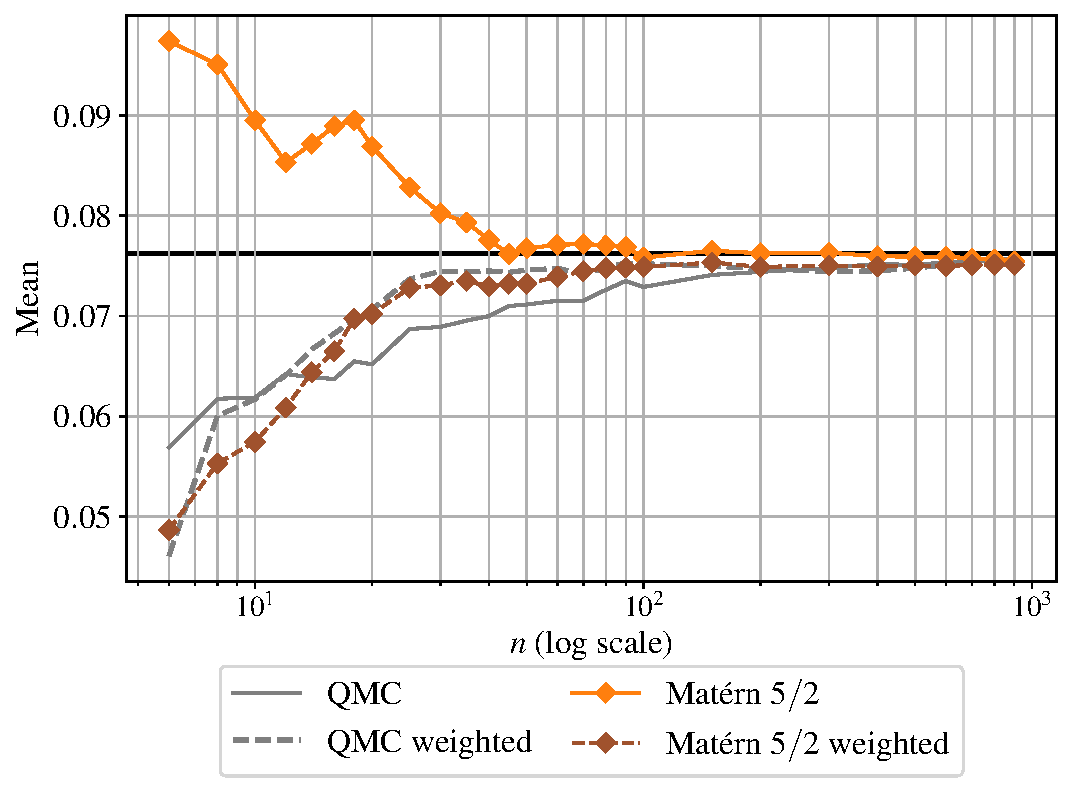
\includegraphics[width=0.48\textwidth]{part2/figures/DCE/analytical_bench/GSobol_10D_(normal_input)_convergence_Matern.pdf}
    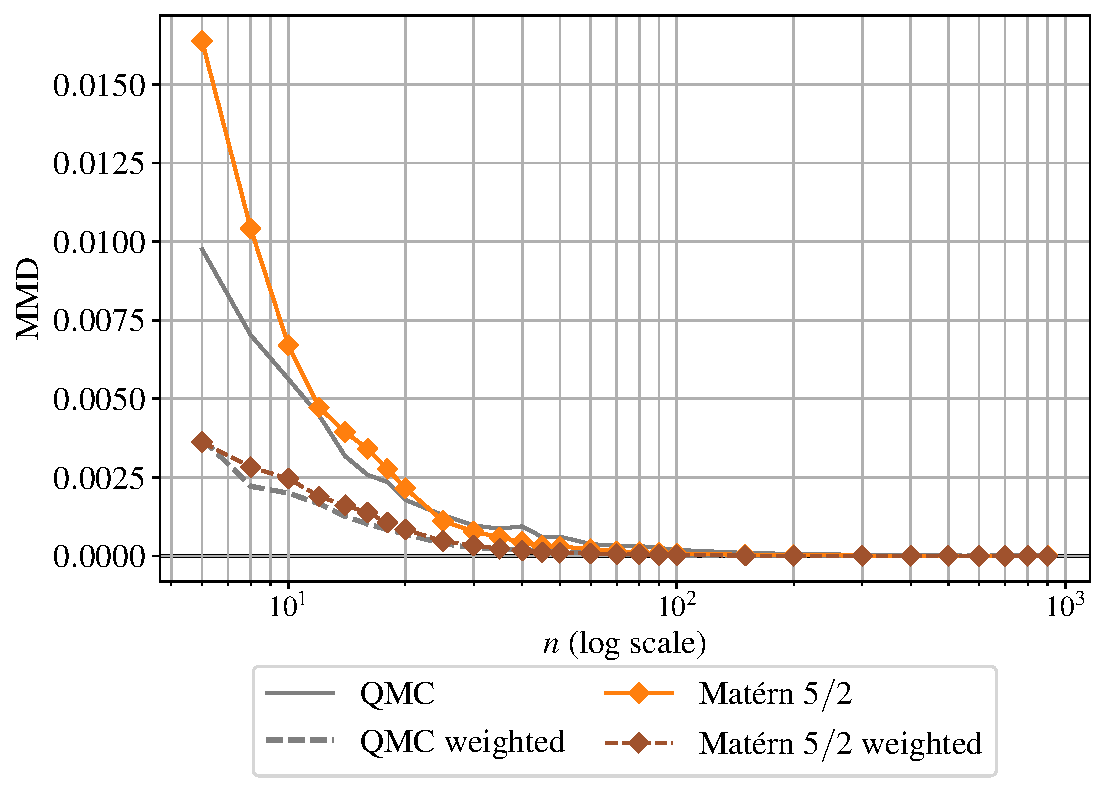
\includegraphics[width=0.48\textwidth]{part2/figures/DCE/analytical_bench/GSobol_10D_(normal_input)_convergence_MMD_Matern.pdf}\\
    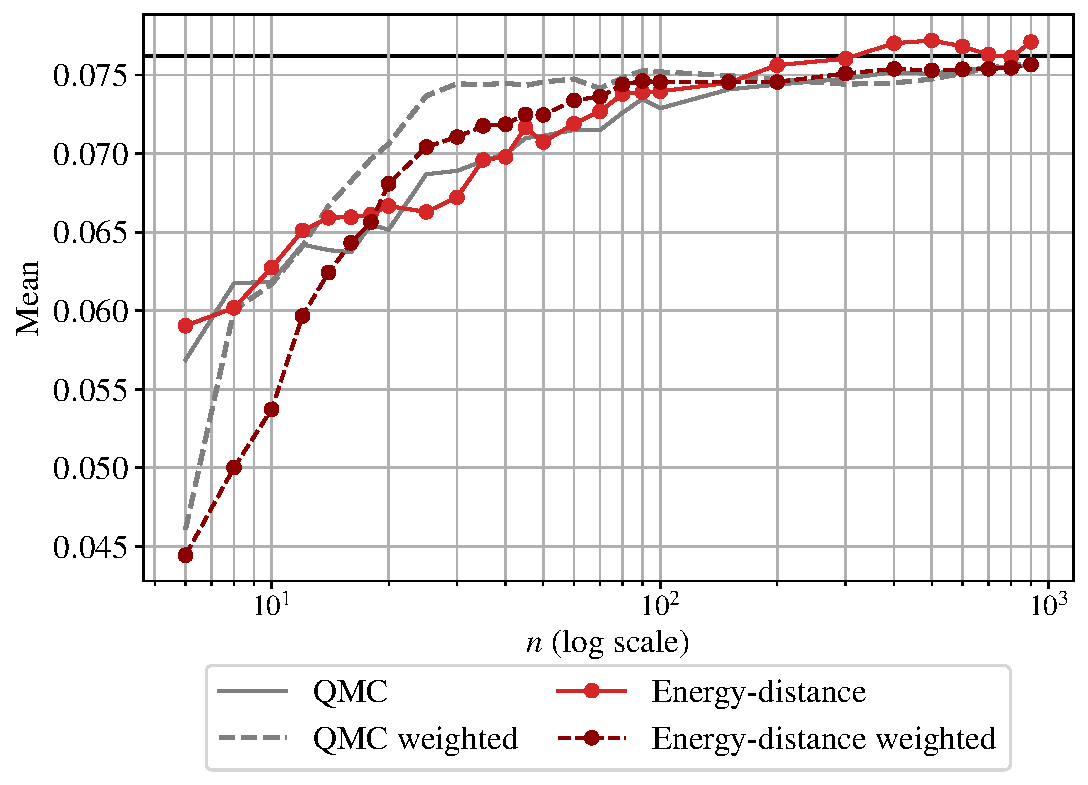
\includegraphics[width=0.48\textwidth]{part2/figures/DCE/analytical_bench/GSobol_10D_(normal_input)_convergence_ED.pdf}
    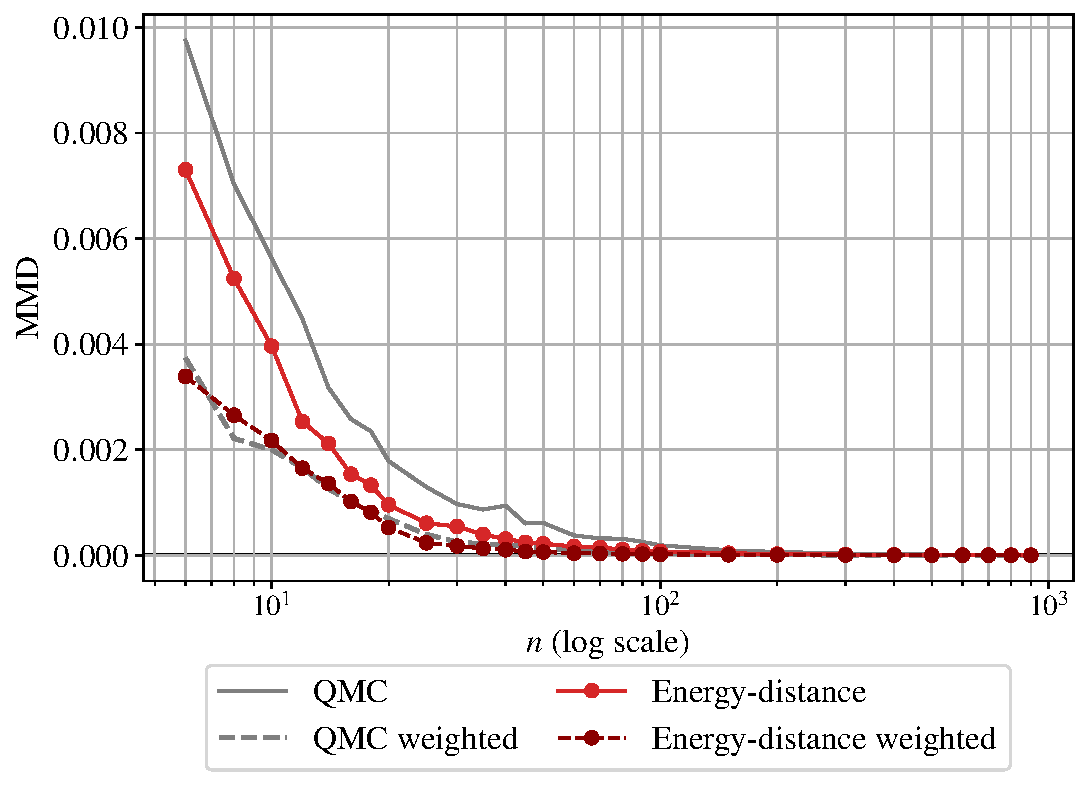
\includegraphics[width=0.48\textwidth]{part2/figures/DCE/analytical_bench/GSobol_10D_(normal_input)_convergence_MMD_ED.pdf}\\
\end{center}
\caption{Analytical benchmark results on the test case \#2.} \label{fig:test case2}
\end{figure}

%----------------------------------------------------------------------%
\subsection{Application to the Teesside wind turbine fatigue estimation}
%----------------------------------------------------------------------%
Let us summarize the mean damage estimation strategies studied in this chapter. 
The diagram represented in \fig{fig:sampling_diagram} describes the different workflows computed. 
The simplest workflow is represented by the grey horizontal sequence. 
It directly subsamples a design of experiments from a large and representative dataset (previously referred to as candidate set). 
This workflow simply estimates the mean damage by computing an arithmetic average of the outputs. 

Alternatively, one can respectively fit a joint distribution and sample from it. 
In our case, this distribution is only known empirically via the candidate set. 
Since its dependence structure is complex (see \fig{fig:envi_pairplot}), a parametric method might fit the distribution poorly (and therefore lead to a poor estimation of the quantity). 
Then, a nonparametric fit using the empirical Bernstein copula (introduced in Subsection~\ref{sec:4ebc}) coupled with a kernel density estimation on each marginal is applied to the candidate set (with the EBC parameter $m=100 > m_{\mbox{MISE}}$ to avoid bias, see \citealp[p.117]{lasserre_2022}). 
The sampling on this hybrid joint distribution is realized with a quasi-Monte Carlo method. 
A Sobol' low-discrepancy sequence generates a uniform sample in the unit hypercube, which can then be transformed according to a target distribution. 
Remember that quasi-Monte Carlo sampling is also sensitive to the choice of a low-discrepancy sequence, each presenting different properties (Sobol', Halton, Faure, etc.). 
Finally, the estimation by an arithmetic mean can be replaced by an optimally weighted mean. 
To do so, optimal weight must be computed, using the formulas introduced in \eq{eq:bq_weights}.

\begin{figure}[!h]
    \centering
    \begin{tikzpicture}
    \node [style=rect] (0) at (0, 0) {Environmental \\SCADA data};
    \node [style=rect] (1) at (3, 0) {Preprocessed \\environmental data};
    \node [style=rect] (2) at (6, 0) {Input design $\mathbf{X}_n$};
    \node [style=rect] (3) at (9, 0) {Output damage $\by_n$};
    \node [style=rect] (4) at (12, 0) {Mean damage};
    \node [style=rect, text width=1.4cm, draw={orange!70}, fill={orange!5}] (5) at (5, -1.75) {Joint \\distribution};
    \node [style=rect, text width=1.4cm, draw={orange!70}, fill={orange!5}] (6) at (11, -1.75) {Optimal weights $\mathbf{w}^{\mathrm{BQ}}_n$};
    \node (9) at (4.25, 0) {};
    \node (10) at (10.25, 0) {};
    \node [style={diag_rect}] (12) at (2, 1.3) {Preprocess \\(detrend and \\filter outliers)};
    \node [style={diag_rect}] (13) at (5, 1.3) {Subsample the data (e.g., using kernel herding)};
    \node [style={diag_rect}] (14) at (8, 1.1) {Evaluate the \\design};
    \node [style={diag_rect}] (15) at (11, 1.1) {Compute \\arithmetic mean};

    \node [style=texte, text width=2.7cm, align=left] at (2.6, -1.2) {Fit a joint distribution (e.g., using EBC)};
    \node [style=texte, text width=2.5cm, align=left] at (7.5, -1.2) {Draw a sample\\ (e.g., using QMC)};
    
    \node [style=texte, text width=2.5cm, align=left] at (10.2, -1.2) {Compute \\optimal\\ weights};
    \node [style=texte, text width=2.5cm, align=left] at (13.5, -1.2) {Compute \\optimally\\ weighted\\ mean};

    \draw [style=arrow] (0) to (1);
    \draw [style=arrow] (1) to (2);
    \draw [style=arrow, in=180, out=-90, {orange!70}] (9.center) to (5);
    \draw [style=arrow, in=-90, out=0, {orange!70}] (5) to (2);
    \draw [style=arrow] (2) to (3);
    \draw [style=arrow] (3) to (4);
    \draw [style=arrow, in=180, out=-90, {orange!70}] (10.center) to (6);
    \draw [style=arrow, in=-90, out=0, {orange!70}] (6) to (4);

    \node [style=dot] at (1.5, 0) {};
    \node [style=dot] at (4.5, 0) {};
    \node [style=dot] at (7.5, 0) {};
    \node [style=dot] at (10.5, 0) {};

    \node [style=dot] at (3.92, -1.2) {};
    \node [style=dot] at (6.15, -1.2) {};
    \node [style=dot] at (9.92, -1.2) {};
    \node [style=dot] at (12.15, -1.2) {};

\end{tikzpicture}
    \caption{Mean damage estimation workflows for the industrial use case. 
    The orange parts represent optional alterations to the workflow: 
    the first one is an alternative to input data subsampling where the underlying distribution is sampled from, 
    the second one improves mean damage calculation by using optimal weights over the output data.}
    \label{fig:sampling_diagram}
\end{figure}


The copulogram in \fig{fig:pairplot_kh_teesside} illustrates the intensity of the computed damages, proportionally to the color scale. 
Note that the numerical values of the damage scale are kept confidential since it models the state of an operating asset.
Before analyzing the performance of the KH on this industrial application, let us notice that the copulogram \fig{fig:pairplot_kh_teesside} seems to be in line with the global sensitivity analysis presented in \cite{murcia_dimitrov_2018} and \cite{li_zhan_2020}. 
In particular, the fact that the scatter plot of mean wind speed vs. turbulence wind speed is the main factor explaining the variance of the output $Y=g(\bX)$. 
Judging from these references, the numerical model does not seem to have a highly effective dimension, however, the input dependence structure is challenging and the damage assessment induces strong nonlinearities (see \eq{eq:wohler}). 

The results presented are compared in the following to a large reference Monte Carlo sample (size $2000$) with a confidence interval computed by bootstrap (see \fig{fig:convergence_teesside}). 
This reference is represented by a horizontal line intersecting with the most converged Monte Carlo estimation.
Once again, the mean damage scale is hidden for confidentiality reasons, but all the plots are represented for the same vertical scale. 
The performance of the KH is good: it quickly converges towards the confidence interval of the Monte Carlo obtained with the reference sample. 
In addition, the Bayesian quadrature estimator also offers a posteriori prediction interval, which can reassure the user. 
The BQ prediction intervals are smaller than the ones obtained by bootstrap on the reference Monte Carlo sample. 

To provide more representative results, note that a set of scale parameters is computed with a Kriging procedure to define the kernel used to compute BQ intervals. 
Since other methods do not generate independent samples, bootstrapping them is not legitimate. 
Contrarily to the other kernels, we observe that the energy-distance kernel presents a small bias with the MC reference for most of the azimuth angles computed in this experiment. 
Meanwhile, combining nonparametric fitting with quasi-Monte Carlo sampling also delivers good results as long as the fitting step does not introduce a bias. 
%In our case, the nonparametric fitting bias is directly related to the empirical Bernstein copula tuning, selected according to the recommendations from \citet{nagler_2017}.    
In our case, any potential bias due to poor fitting would be the result of a poorly tuned empirical Bernstein copula. 
Fortunately, \cite{nagler_2017} formulated recommendations regarding how to tune empirical Bernstein copulas. 
We follow these recommendations in the present work.



\begin{figure}[!h]
\begin{center}
    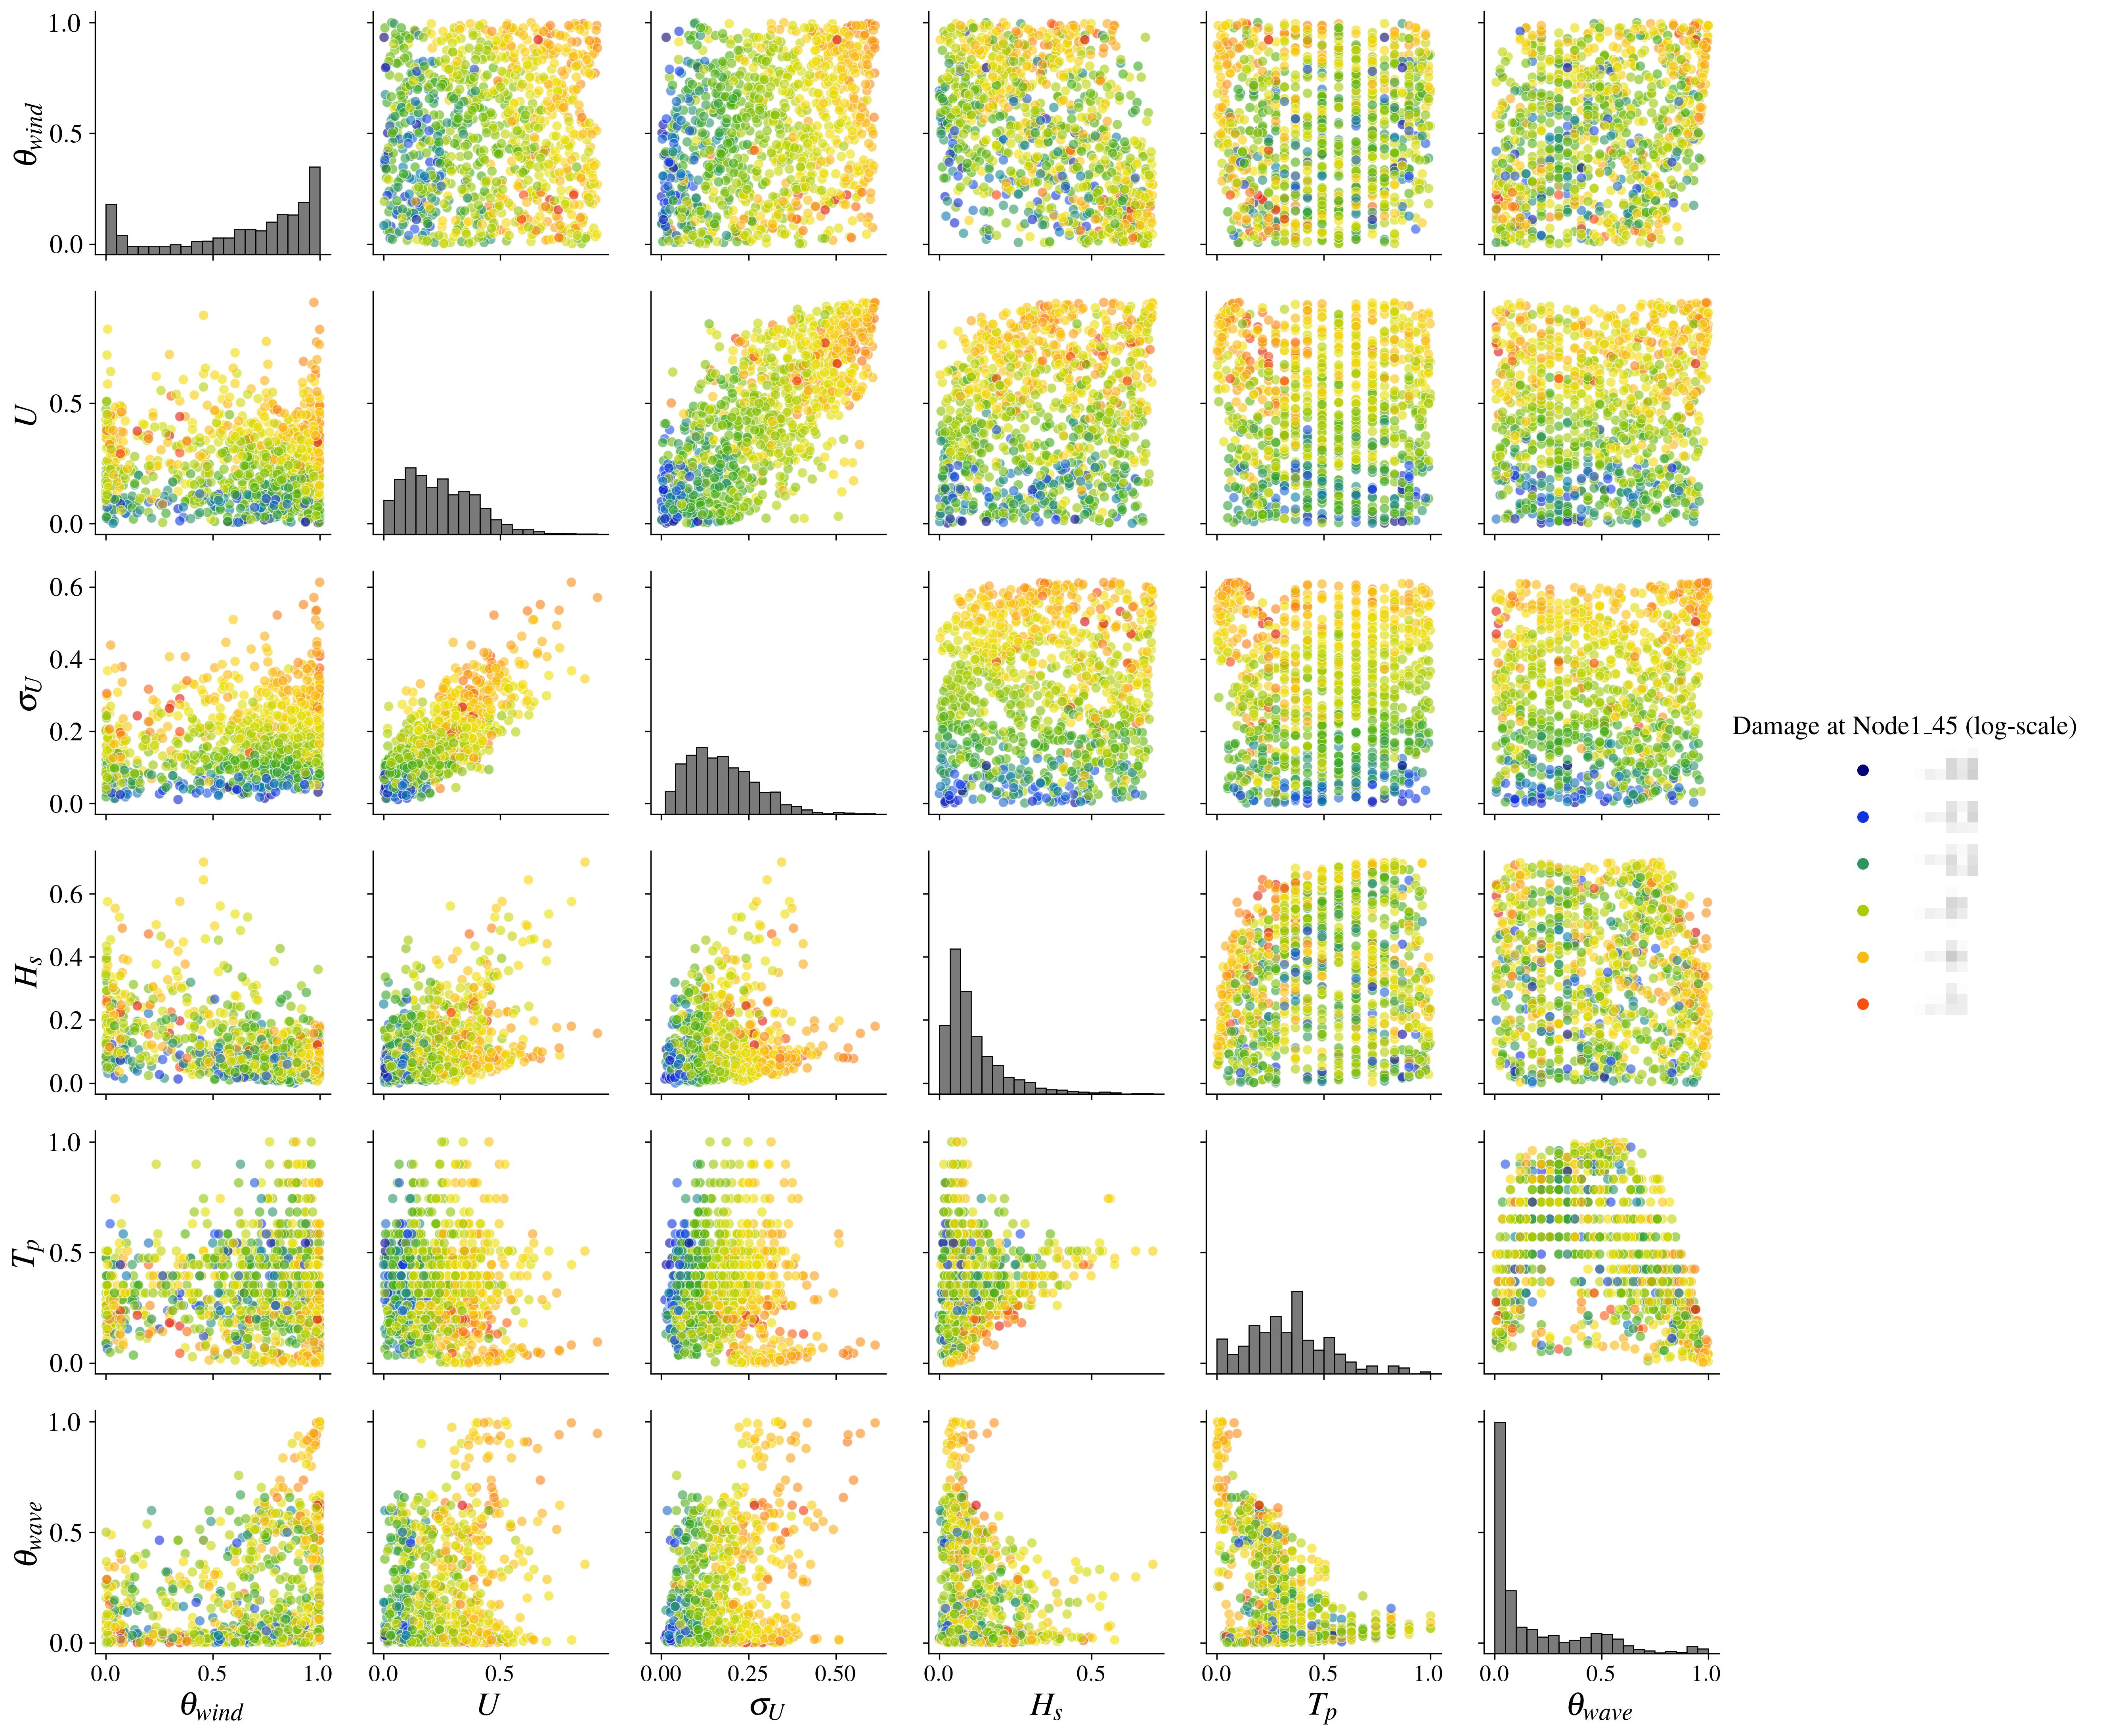
\includegraphics[width=\textwidth]{part2/figures/DCE/teesside/kh_output_pairplot.jpg}
\end{center}
\caption{Copulogram of the kernel herding design of experiments with corresponding outputs in color (log-scale) on the Teesside case ($n = 10^3$). 
The color scale ranges from blue for the lowest values to red for the largest.
Marginals are represented by histograms (diagonal), the dependence structure with scatter plots in the ranked space (upper triangle). 
Scatter plots on the bottom triangle are set in the physical space.} \label{fig:pairplot_kh_teesside}
\end{figure}

\begin{figure}[!h]
\begin{center}
    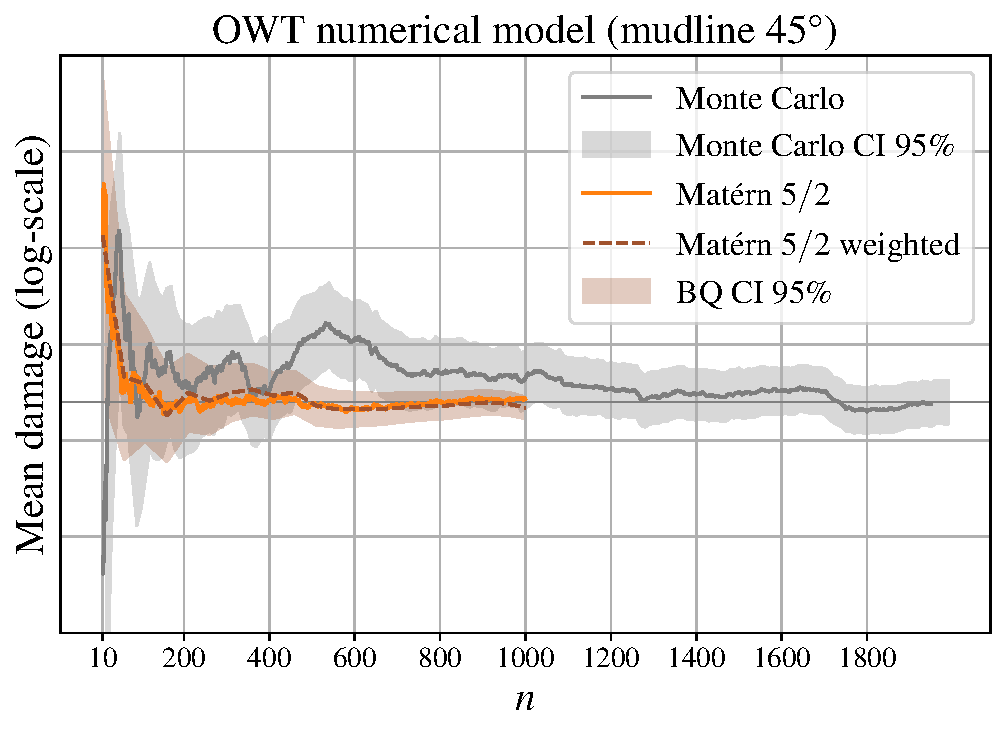
\includegraphics[width=0.49\textwidth]{part2/figures/DCE/teesside/log_convergence_MaternNode1_45.pdf}
    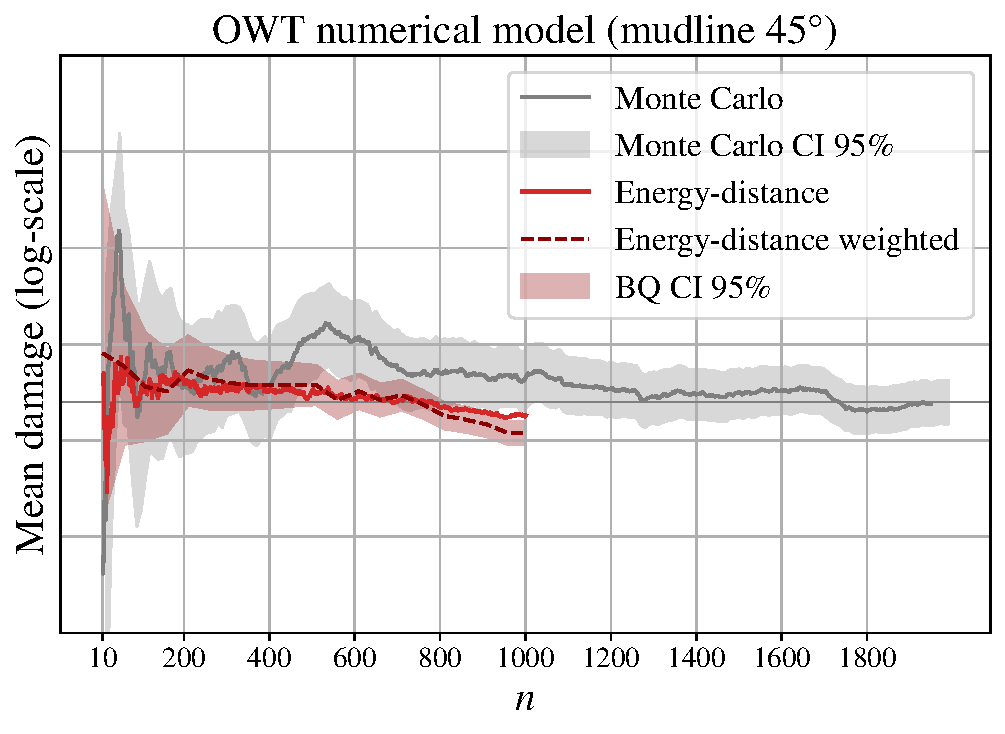
\includegraphics[width=0.49\textwidth]{part2/figures/DCE/teesside/log_convergence_EnergyNode1_45.pdf}
    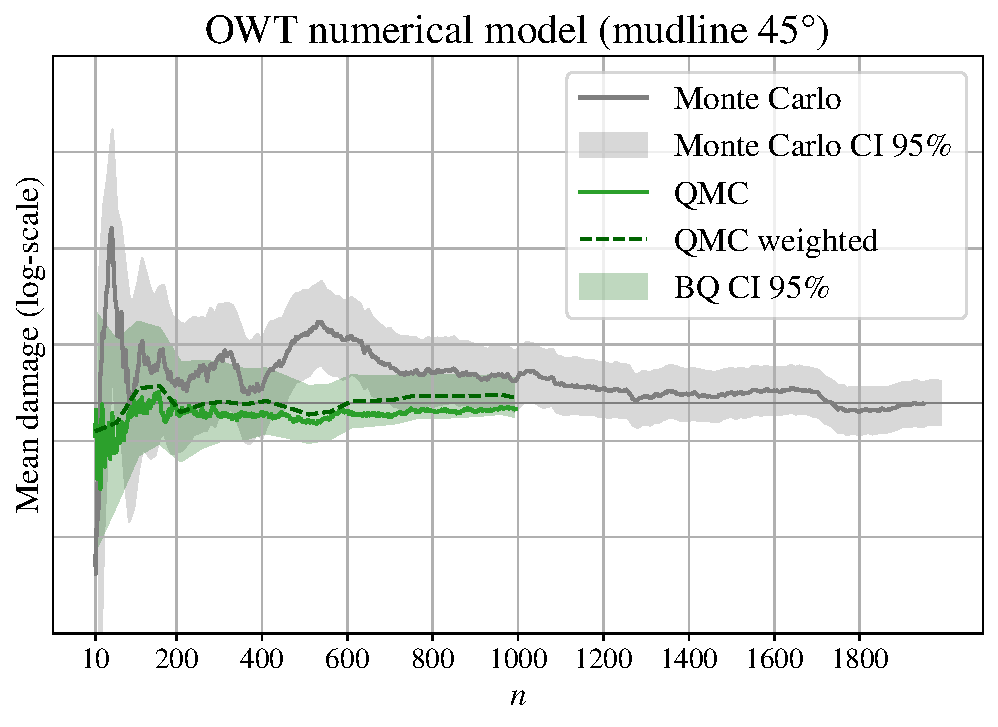
\includegraphics[width=0.49\textwidth]{part2/figures/DCE/teesside/log_convergence_QMCNode1_45.pdf}
\end{center}
\caption{Mean estimation convergence (at the mudline, azimuth $\theta=45~\mathrm{deg.}$) on the Teesside case. Monte Carlo confidence intervals are all computed by bootstrap.} 
\label{fig:convergence_teesside}
\end{figure}


%============================================================%
%============================================================%
\section{Conclusion}\label{sec:sec45}
%============================================================%
%============================================================%

Wind energy assets are subject to highly uncertain environmental conditions. 
Uncertainty propagation through numerical models is performed to ensure their structural integrity (and energy production). 
For this case, the method recommended by the standards (regular grid sampling) is intractable for even moderate-fidelity simulators. 
In practice, such an approach can lead to poor uncertainty propagation, especially when facing simulation budget constraints.

In the present chapter, a real industrial wind turbine fatigue estimation use case is investigated, considering site-specific data. 
As a perspective, other sites with different environmental conditions could be studied. 
This use case induces two practical constraints: first, usual active learning methods are hard to set up on such a model (mainly due to the nonlinearity of the variable of interest), and they restrict the use of high-performance computing facilities; second, the input distribution of the environmental conditions presents a complex dependence structure which is hard to infer with common parametric approaches. 

In this work, the association of kernel herding sampling with Bayesian quadrature for central tendency estimation is explored theoretically and numerically. 
This method fits with the practical constraints induced by the industrial use case. 
To be more specific, the kernel herding method easily subsamples the relevant points directly from a given dataset (here, from the measured environmental data). 
Moreover, the method is fully compatible with intensive high-performance computer use. 
Moreover, the present work outlined an upper bound based on the maximum mean discrepancy (MMD) on numerical integration absolute error. 
Kernel herding and Bayesian quadrature both aim at finding the quadrature rule minimizing the MMD, and therefore the absolute integration error. 
The numerical experiments confirm that the MMD is an appropriate criterion since it leads to results being better or equivalent to quasi-Monte Carlo sampling. 
Finally, the proposed numerical benchmark relies on a Python package, called \texttt{\href{https://efekhari27.github.io/otkerneldesign/master/index.html}{otkerneldesign}}, which implements the methods and allows anyone to reproduce the results. 

The limits of the proposed method are reached when the input dimension of the problem increases, requiring a larger candidate set and therefore a larger covariance matrix. 
Moreover, the numerical experiments show that the method can be sensitive to the choice of the kernel and its tuning (although good practices can be derived). 
From a methodological viewpoint, further interpretation of the impact of the different kernels could be explored. 
Besides, extensions of kernel herding sampling for quantile estimation could be investigated, in a similar fashion as the work on randomized quasi-Monte Carlo for quantiles proposed by \cite{tuffin_2019}. 
Kernel herding could also be used to quantize conditional distributions, using the so-called ``conditional kernel mean embedding'' concept reviewed by \cite{sullivan_2020}. 
Finally, regarding the industrial use case, the next step should be to perform a reliability analysis by considering another group of random variables (related to the wind turbine) or to explore the possibilities offered by reliability-oriented sensitivity analysis in the context of kernel-based indices, as studied in \citet{marrel_chabridon_2021}.

